\chapter{Near-Field Electrospinning as an Affordable Way to Gain Spatial Control} % Main chapter title

\label{Chapter:2}

%----------------------------------------------------------------------------------------
%	SECTION 1
%----------------------------------------------------------------------------------------
\section{Review of Polymer Solutions for NFES with Spatial Control}

Near-field electrospinning (NFES) is identified to be a technique able to fabricate polymer nano and micro fibers with accurate placement. \cite{He2017} In the past years (2006-2020) \cite{Helgeson2007,
  Yang2019,Fattahi2017,Shin2019,Wang2015,Parajuli2016,Zheng2010,Fuh2011,Dalton2015,
  Ru2014,Xue2014,Wang2017,Xu2014,Liu2013,Pan2014,Canton2014,Chakraborty2009,Gupta2007,
  He2018,Zhou2011,Chen2013,Williams2018,Choi2017,Pan2019,Lei2015,Lim2019,Park2020,
  Fuh2012,Flores2017,Chang2010,Xu2019,Zhang2019,Shin2018,Fuh2015,Nagle2019,Zheng2012,
  Kameoka2003a,Liu2014,E.King2019,Hochleitner2017,Madou2011,Jiang2018,Husain2016,
  ElectrospinTech2015,Brown2011,Kolan2018,Chang2011,Beachley2011,Camillo2013,Kameoka2003,
  Bu2012,Lee2012,Huang2015,Coppola2020,CisquellaSerra2019,Ruggieri2013,Hochleitner2014,
  Zhu2016,Brown2014,Chang2008,Sonntag2020,Kim2018,Deng2020,Han2019,George2020,Sun2006a,
  Pan2015,Shen2016,Strauss2019,Fuh2013,Sarkar2007,You2017,Wang2018a,Zheng2014,Song2015,
  GaofengZheng2010,Liu2015a,Min2013,Luo2016,Yousefi2019,Cardenas2017,Coppola2014}, several polymer solutions have been successfully electrospun into fibers through several variants of the conventional NFES process. Each NFES variant intended to tailor the process parameters in order to improve the fibers' properties. 

Near-field electrospinning (NFES) is known as a versatile nano-fabrication technique, suitable for several applications such as tissue engineering, chemical sensing, filtration, energy storage, besides others (see Figure \ref{fig:synthesesAndApplicationsOfNanofibers}). Fast developments in electrospinning has been observed in recent years. However, this process is limited by the electric field wiping instability effects during polymer deposition. This leads to a major challenge: how to surpass this limitation of planar two-dimensional prints. The current trend in this area lies on the research of new materials, techniques to increase precision patterning in NFES systems.

\begin{figure}[!th]
\centering
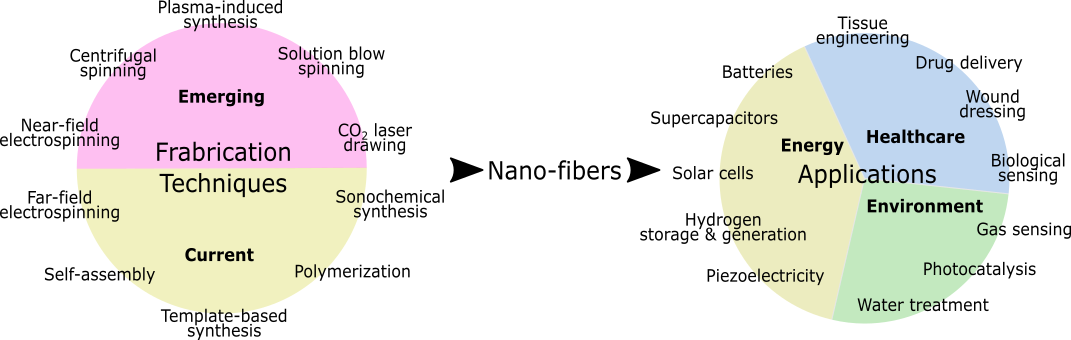
\includegraphics[width=\textwidth]{./Figures/synthesesAndApplicationsOfNanofibers.png}
\decoRule
\caption[Syntheses and Applications of Nanofibers]{Syntheses and Applications of Nanofibers. Adapted from \cite{Kenry2017}}
\label{fig:synthesesAndApplicationsOfNanofibers}
\end{figure}

Even though electrospinning is an old invention \unskip~\cite{527120:12073288}, it is currently a trending topic among researchers \unskip~\cite{527120:12073453,527120:12073495,527120:12073496}. One of the reasons electrospinning is to be studied is its potential to fabricate polymer nano fibers from a variety of polymers. The technique allows the production of thin continuous fibers with ease, with micro and sub-micrometer diameters, which is something difficult to achieve by other techniques. Furthermore, the basic setup can be modified with ease to fabricate different fibers with diversified functionalities from different materials. The produced fibers can be aligned or unaligned. Besides, the electrospinning equipment is inexpensive and of small size, compared to the equipment of standard spinning techniques\unskip~\cite{527120:12073538}. On the other hand, the understanding of the electrospinning process has improved in the last years.

Current literature dictates the typical spinning setup is comprised by three main components: a polymer reservoir, a fiber collector, and some way to dispense the fibers onto the collector. The spinning process is an electro-hydrodynamic (EHD) technique that yields continuous polymer fibers. Other EHD techniques are spraying and atomization which produce polymer droplets and polymer particles respectively, seeFigure~\ref{f-02e0e3cf88d6}.

\bgroup
%\fixFloatSize{images/514dfac6-849d-4905-8e40-7adfafc93b5f-uimg_ehd_techniques.png}
\begin{figure}[!htbp]
\centering \makeatletter\IfFileExists{./images/514dfac6-849d-4905-8e40-7adfafc93b5f-uimg_ehd_techniques.png}{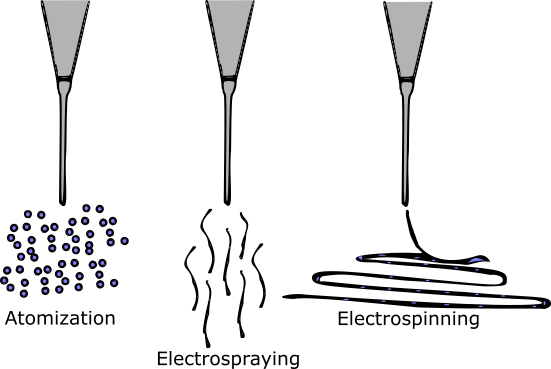
\includegraphics[scale=0.65]{./images/514dfac6-849d-4905-8e40-7adfafc93b5f-uimg_ehd_techniques.png}}{}
\makeatother 
\caption{{Electrohydro-dynamic techniques}}
\label{f-02e0e3cf88d6}
\end{figure}
\egroup

\subsection{Stretching forces}

\subsubsection{Electric Field}Electrospinning (electrostatic fiber spinning) is a fiber fabrication approach that implements an electric field to produce fibers by applying an electrical potential difference between the syringe needle and the collector. With the influence of high electric fields, the fibers are prone to brake into separate layers due to the whipping instabilities as the jet travels to the substrate. The instability can be mitigated by adding additional ring electrodes between the spinneret and the grounded collector. \unskip~\cite{527120:13915304}

The typical electrospinning setup applies an electrostatic charge to the polymer fluid at the tip of the needle nozzle, which results in the formation of the Taylor cone \unskip~\cite{527120:13659828}, from which a single polymer jet is ejected to the grounded collector. From the Taylor cone, the supplied polymer jet (typically a polymer solution) accelerates and reduces in diameter. The fiber finally develops upon complete solvent evaporation. Electrospun fibers are prone to splitting with the increase in acceleration due to high applied voltages, where multiple fibers are produced in a process known as electrospraying \unskip~\cite{527120:13659925}.

The electrospinning process starts with charging a polymer solution droplet. When a polymer solution is administrated with a syringe pump, solution droplets will fall under the influence of gravity. The solution dripping stops when the electric field is strong enough to break the solution's surface tension, causing the droplet to change shape forming a jet\unskip~\cite{527120:12033655}.

Shin et al. \unskip~\cite{527120:13659926} reported that the growth of the whipping instability is one important element within the electrospinning technique. As detailed in Shin's work, weak electric fields produce a single uniformly thinning jet, and at strong electric fields the jet becomes unstable after traveling a short distance.


\paragraph{High voltage power supply: DC \& AC - }Direct current (DC) is typically used in electrospinning with the electrons flowing in one direction. Alternate current (AC) implementations are also studied as the AC creates a change in the direction of the current flow. Kessick et al.\unskip~\cite{527120:13444381} demonstrated the implementation of AC power supplies in the production of polymer fibers.

The AC electrospinning setup is similar to that for the DC variant. AC electrospinning apparatus do not require a grounded collector as the current alternates. In AC, the produced fibers are prone to carry an electric charge, while those generated shortly after have an opposite charge. The difference in charges lead the fibers to discharge on each other, creating an aerogel plume of fibers\unskip~\cite{527120:16885570}. The optimal AC frequency depends on the materials used and is typically within  $50Hz $ and  $1kHz $\unskip~\cite{527120:13443405}.

The AC technique has been studied for drug loaded related applications. Balogh et al. \unskip~\cite{527120:13445177} compared fibers fabricated by DC and AC spinning techniques. Their work reports that AC and DC electrospinning can produce fibers with all three polymers, where the AC process allowed the implementation of faster flow rates than in the DC setup. The DC electrospinning technique generated fibers with a maximum flow rate of 5 $ml/h $; on the other hand, the AC setup allowed an increase in flow rate up to 40 $ml/h $.


\subsubsection{Centrifugal force}The spinning processes require the implementation of a force to break the polymer source into a polymer jet. Centrifugal spinning intends to produce fibers by the use of a rotating polymer source. The centrifugal force generated from typical rotatory speeds above $2000 \textrm{ rpm}$, results in fiber formation. \unskip~\cite{527120:13535559,527120:13535561}.


\bgroup
%\fixFloatSize{./images/19c94c11-1ae0-47bd-95ef-4dc5ceedc20d-uimg_gyro_es.png}
\begin{figure}[!htbp]
\centering \makeatletter\IfFileExists{./images/19c94c11-1ae0-47bd-95ef-4dc5ceedc20d-uimg_gyro_es.png}{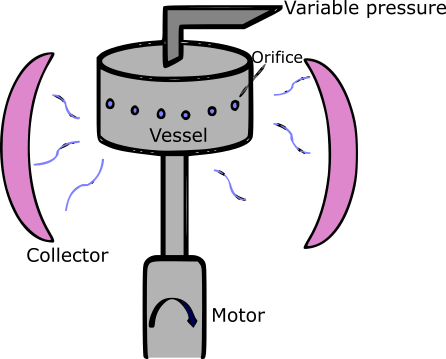
\includegraphics[scale=0.65]{./images/19c94c11-1ae0-47bd-95ef-4dc5ceedc20d-uimg_gyro_es.png}}{}
\makeatother 
\caption{{Typical setup used in pressurized gyration processes}}
\label{f-7cf6ac702e28}
\end{figure}
\egroup
The centrifugal force technique has been applied to polymer solutions and melts. This approach is used in applications were the precise deposition of the fibers is not relevant and production rate is to be maximized \unskip~\cite{527120:13535894}.  Efforts in centrifugal spinning are focused on drug delivery applications. Zander \unskip~\cite{527120:13535977} fabricated polycaprolactone (PCL) fibers using the solution and melt variants of the centrifugal approach. Zander's fibers were produced with rotatory speed between $3000$ and $18000 \textrm{ rpm}$ obtaining $10 \mu m $ diameters. 

On the other hand, PCL and PVP fibers were generated by Amalorpava et al. \unskip~\cite{527120:13536089}.  Amalorpava achieved sub micron/size fiber diameters for drug release purposes and bacteria growth inhibition properties. Literature\unskip~\cite{527120:13536446} has shown that centrifugal approach has a simple setup that promises a large scale fabrication of fibers.

In some cases the centrifugal force implementations and pressurized gyration can be combined with an electric field. The implementation of two stretching forces (centrifugal and electrical forces), can help solvent evaporation\unskip~\cite{527120:13536560}. Centrifugal electrospinning implements the same setup as the standard centrifugal spinning with the addition of a high voltage power supply between the rotating dispensing nozzle and the collector. The combined method has been proven to yield parallel fibers\unskip~\cite{527120:13536841,527120:13536900,527120:13537392,527120:13537393} at a higher rate \unskip~\cite{527120:13536841,527120:13536900} than the standard electrospinning approach.



\subsubsection{Blowing forces}Nano-fibers can be produced with the implementation of pressurized gas with a polymer solution. The setup used for blow spinning is similar to the one used in coaxial electrospinning, where the polymer precursor is dispensed at a controlled rate. Unlike traditional electrospinning, in the solution blow spinning setup the needle nozzle applies pressurized gas to the polymer solution through an outer spinneret\unskip~\cite{527120:13538056}, see Figure~\ref{f-92361290d8c3}. 


\bgroup
%\fixFloatSize{./images/87246522-4cf1-491f-a45f-cda541854d72-uimg_blow_es.png}
\begin{figure}[!htbp]
\centering \makeatletter\IfFileExists{./images/87246522-4cf1-491f-a45f-cda541854d72-uimg_blow_es.png}{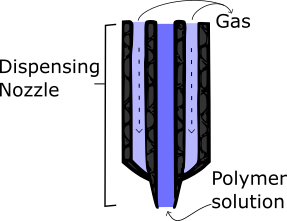
\includegraphics[scale=0.65]{./images/87246522-4cf1-491f-a45f-cda541854d72-uimg_blow_es.png}}{}
\makeatother 
\caption{{Dispensing nozzle used for solution blow spinning or melt blowing. \unskip~\protect\cite{527120:13538056}}}
\label{f-92361290d8c3}
\end{figure}
\egroup
Poly(lactic acid) (PLA) fibers have been produced by solution blow spinning. Oliveira et al. \unskip~\cite{527120:13539278} fabricated fibers from $6 wt\% $ PLA solutions with progesterone for live stock reproductive cycle regulation applications. On the other hand, Souza et al.\unskip~\cite{527120:13538056} conducted a study to compare the standard electrospinning and the solution blow spinning techniques. Poly(3-hydroxybutyrate-co-3-hydroxyvalerate) were fabricated by both methods. The fibers produced by traditional electrospinning had thicker diameters and the size uniformity was higher in the fibers produced by solution blow spinning. The experimental setup requires a coaxial needle nozzle with a pressurized gas flow along with a potential difference between the dispensing needle and the grounded collector.



\subsubsection{Mechanical force}
\bgroup
%\fixFloatSize{./images/23a9bc42-4d02-4a78-a907-23aeeb2de68a-uimg_meches_process.png}
\begin{figure*}[!htbp]
\centering \makeatletter\IfFileExists{./images/23a9bc42-4d02-4a78-a907-23aeeb2de68a-uimg_meches_process.png}{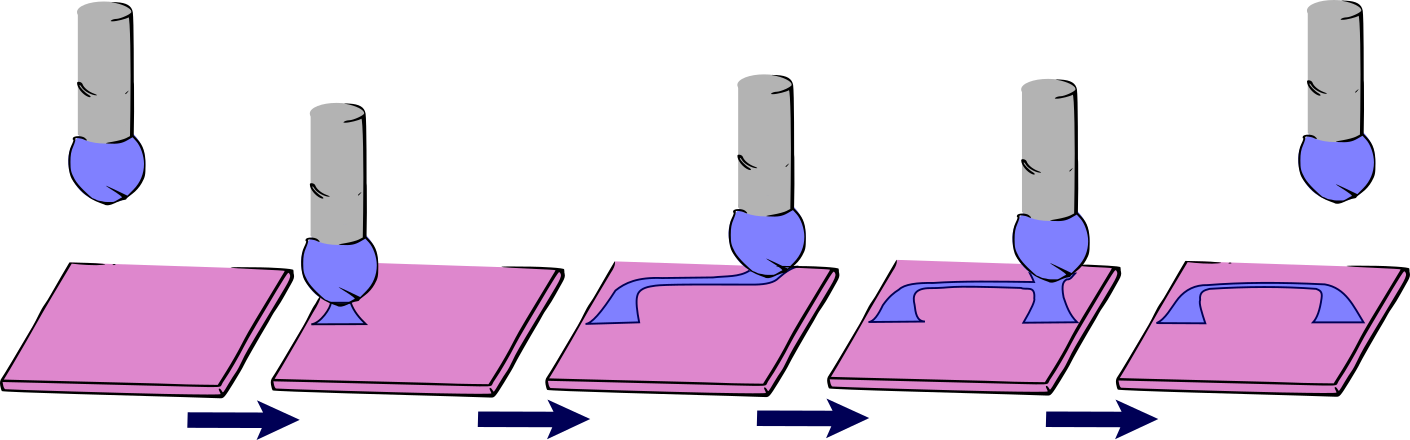
\includegraphics[scale=0.35]{./images/23a9bc42-4d02-4a78-a907-23aeeb2de68a-uimg_meches_process.png}}{}
\makeatother 
\caption{{Typical mechanical fiber drawing process}}
\label{f-432d16f420fb}
\end{figure*}
% First the needle makes contact with the substrate to break the polymer drop. Then the needle leaves the substrate and the collector moves to create and deposit the fiber. Once the fiber is written the needle makes contact witht the collector to fix the fiber deposition.

\egroup
Mechanical drawing comprises the simple technique to produce fibers by stretching the polymer solution with a glass pipette. \unskip~\cite{527120:14024998} Nevertheless, the drawing technique is not scalable or with practical complications. \unskip~\cite{527120:14025041} Touch-spinning methods have been developed to introduce a scalable technique for the production of nano fibers where the fiber is created by stretching the polymer precursor with a moving collector, as depicted in Figure~\ref{f-432d16f420fb}. Touch-spinning is another mechanical technique that comprises a moving stage with an embedded glass rod (Figure~\ref{f-f17259e76303}), where a polymer solution is supplied from a syringe needle such that the tip of the glass rod makes contact with the polymer solution as it rotates, creating fibers. The rotation stretches the fiber, causing the fiber to increase in length and decrease in diameter. The increase in length causes the fiber surface are to increase and therefore making the polymer solution solvent to volatilize, ending with a dry fiber within the collector.


\bgroup
%\fixFloatSize{./images/c33e7bfe-18c6-4765-834e-a85f12cd2621-uimg_touch_process.png}
\begin{figure*}[!htbp]
\centering \makeatletter\IfFileExists{./images/c33e7bfe-18c6-4765-834e-a85f12cd2621-uimg_touch_process.png}{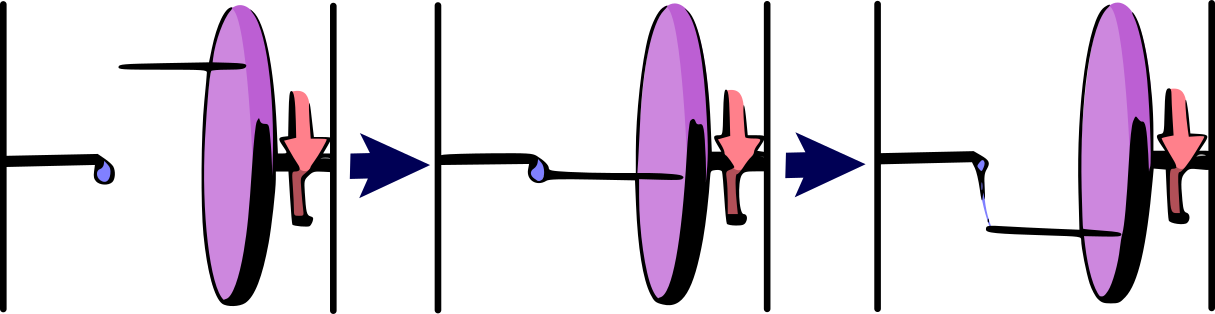
\includegraphics[scale=0.45]{./images/c33e7bfe-18c6-4765-834e-a85f12cd2621-uimg_touch_process.png}}{}
\makeatother 
\caption{{Touch-spinning technique.}}
\label{f-f17259e76303}
\end{figure*}
% First rod is attached to a rotating stage and a polymer solution droplet is administrated through a needle. Then the rotating rod 'touches' the polymer precursor. Finally, as the rod rotates, the polymer solution is stretched and creates a fiber between the rod and the needle.

\egroup
The touch spinning technique implies that the fiber diameter can be controlled by the moving collector's speed and the polymer solution concentration. The main difference lies on the fact that the touch spinning method implements mechanical control to manipulate and stretch the fibers during the fabrication process, guiding the fiber in the collector enabling better control over fiber alignment.\unskip~\cite{527120:14091959}



\subsubsection{Microfluidic forces}The microfluidic spinning technique manipulates and controls the polymer solution in networks of micrometer channels. The channel network are typically embedded in a microfluidic chip, where the solution deposition rate is controlled by active components (pumps and valves) with a computer. Cheng et al. \unskip~\cite{527120:13656236} compared and combined the microfluidic spinning and electrospinning techniques. Heterogeneous materials and cell patterning within a single microfiber can be designed by the integration of microfluidic channels. Therefore, microfluidic spinning is more suitable for cell encapsulation and tissue regeneration and tissue engineering \unskip~\cite{527120:13656236}.

On the other hand, Kang et al. \unskip~\cite{527120:13656548} managed to fabricate micro fibers by imitating the "silk spinning" process of spiders. Kang's micro fibers properties were modified using a microfluidic system with a programmable flow control (See Figure~\ref{f-c0beae2757bf}). The current microfluidic spinning approach is not scalable to a large fiber production, however it enables the fabrication of high-complex fibers that are not easily achieved by other methods.


\bgroup
%\fixFloatSize{./images/efb1d6af-4f1a-4c34-9726-b0015b59e112-uimg_microfluid_setup.png}
\begin{figure}[!htbp]
\centering \makeatletter\IfFileExists{./images/efb1d6af-4f1a-4c34-9726-b0015b59e112-uimg_microfluid_setup.png}{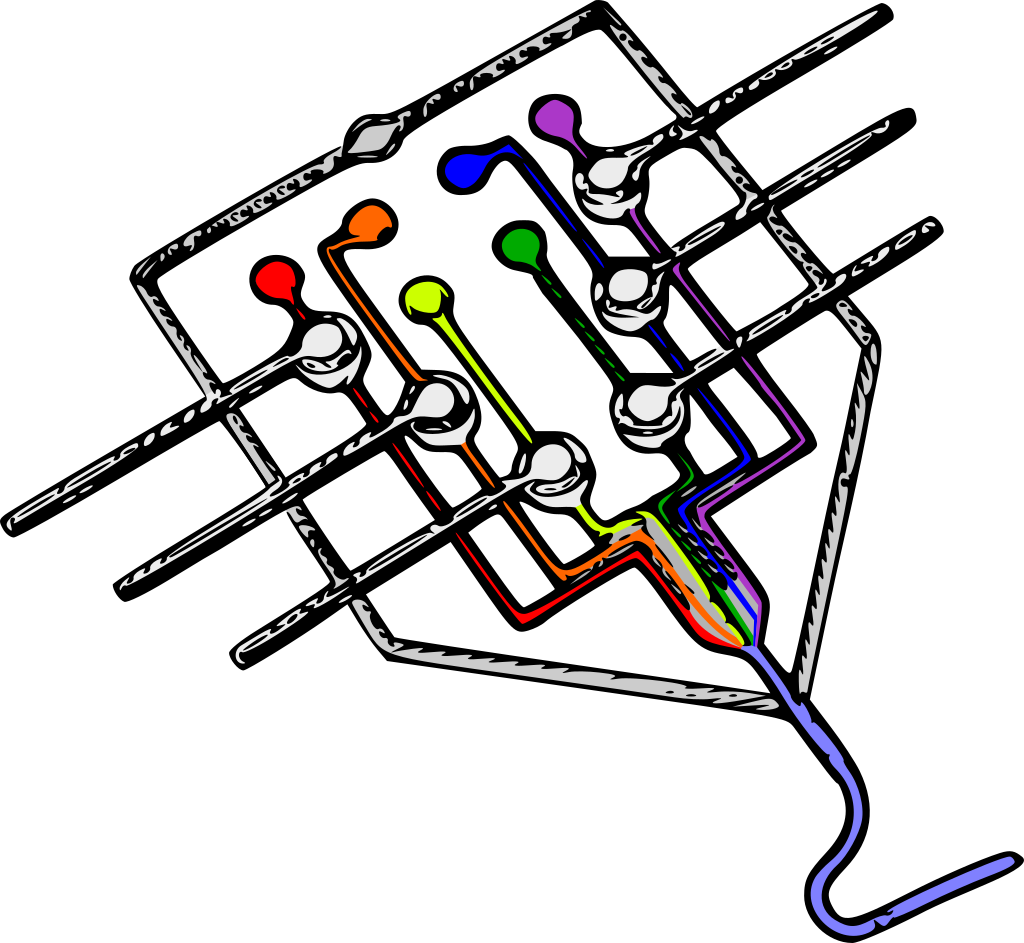
\includegraphics[scale=0.99]{./images/efb1d6af-4f1a-4c34-9726-b0015b59e112-uimg_microfluid_setup.png}}{}
\makeatother 
\caption{{Microfluidic device used by Kang et al.\unskip~\protect\cite{527120:13656548}}}
\label{f-c0beae2757bf}
\end{figure}
\egroup
Microfluidic techniques offer the possibility to embed several components into a single fiber, where each component can be released at different parts of the fiber. 



\subsection{Dispensing nozzle}Unlike traditional electrospinning, coaxial electrospinning (co-electrospinning) requires de implementation of a dual needle nozzle, where one needle is nested concentrically inside another needle, see Figure~\ref{f-4a5ffd16c3ab}\unskip~\cite{527120:13914792,527120:13914793}. The purpose of the co-electrospinning setup is to produce core/shell fibers, unlike mono axial electrospinning that yields monolithic fibers. Sun et al. \unskip~\cite{527120:13914312}. Addressed electrospinning setups, where both the core and shell are comprised by PEO (poly(ethylene oxide)) and for a PEO shell with a poly(dode-cylthiophene) core. Sun et al. state that co-electrospinning has the potential to extend the range of materials that can be used for electrospinning. The shell solution can be modified to make the core solution spunable. It was also discovered that non-spunable solutions can by implemented as shell solutions in conjunction with a spunable core solution. \unskip~\cite{527120:13914968}


\bgroup
%\fixFloatSize{./images/afe7da25-1366-4b1e-bf1a-0594eb2eaa88-uimg_nozzle.png}
\begin{figure}[!htbp]
\centering \makeatletter\IfFileExists{./images/afe7da25-1366-4b1e-bf1a-0594eb2eaa88-uimg_nozzle.png}{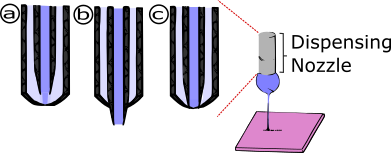
\includegraphics[scale=0.80]{./images/afe7da25-1366-4b1e-bf1a-0594eb2eaa88-uimg_nozzle.png}}{}
\makeatother 
\caption{{Needle configurations in coaxial electrospinning. (a) the outer needle encasing the inner; (b) the inner needle protruding from the outer; (c) both needles inline with each other;}}
\label{f-4a5ffd16c3ab}
\end{figure}
\egroup
Some advantages of co-electrospinning setups are the breaking of the polymer drop surface tension, initiating the jet burst from the spinneret nozzle. On the other hand, as the morphology and shape of the fibers depend on the polymer solution properties, the use of a co-axial nozzle allows the modification of the material properties by producing bubbles, scaffolds and particles. \unskip~\cite{527120:13914748,527120:13914750}. As in conventional NFES, in co-electrospinning, the needle tip is connected to a high voltage power supply with a grounded collector.



\subsection{Polymer Reservoir (Polymer Melt \& Polymer Solution)}Electrospinning processes can be classified based on the type of polymer reservoir. As Brown et al. \unskip~\cite{527120:13445499} discussed, the polymer melt is equivalent to the polymer solution electrospinning. The use of a polymer melt increases the complexity of the process, because the nozzle syringe and spinneret required to be heated to maintain the polymer in a liquid state. The fibers produced in melt spinning are typically found to have larger diameters than those from the polymer solutions due to the higher viscosity of a polymer melt. The apparatus used by Brown et al. \unskip~\cite{527120:13445499} is depicted in Figure~\ref{f-bfd139aecf8f}.


\bgroup
%\fixFloatSize{./images/9d06b4aa-134c-4fd6-bbf3-1ced4ac95046-uimg_metl_setup.png}
\begin{figure}[!htbp]
\centering \makeatletter\IfFileExists{./images/9d06b4aa-134c-4fd6-bbf3-1ced4ac95046-uimg_metl_setup.png}{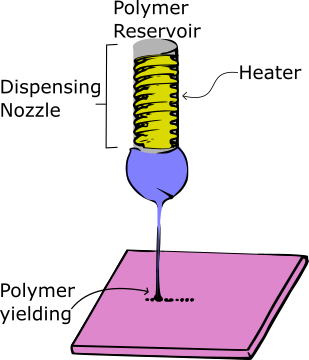
\includegraphics[scale=0.70]{./images/9d06b4aa-134c-4fd6-bbf3-1ced4ac95046-uimg_metl_setup.png}}{}
\makeatother 
\caption{{Typical Melt Electrospinning Setup}}
\label{f-bfd139aecf8f}
\end{figure}
\egroup
Despite the added complexity and thicker diameters, the melt electrospinning technique is safer to be performed on larger scales as it does not have the need to handle volatile solvents. Therefore, polymer melt reservoirs get rid of any solvent contamination. The first report of a melt electrospun drug delivery system came from Nagy et al. \unskip~\cite{527120:13445555}, who prepared fibers by melt electrospinning of Eudragit EPO with carvedilol. The drug and polymer were melted and mixed to form a homogeneous solid mixture prior to spinning. The melt-spun fibers reached diameters of 5{\textendash}30 $\mu m $, compared to 300{\textendash}1000 $nm $ diameters produced from solution-spun fibers\unskip~\cite{527120:13445555}.

Balogh et al.'s work has built on this idea by blending plasticizes with the polymer Eudragit EPO and carvedilol active ingredient.\unskip~\cite{527120:13445752} The plasticizes Triacetin, Tween 80 and Polyethylene Glycol were investigated in order to reduce the melting point of the polymer-drug mixture. A lower temperature is desirable to minimize the degradation of the drug.

Lian and Meng\unskip~\cite{527120:13445754} performed a comparison of poly(\ensuremath{\varepsilon }-caprolactone) (PCL) fibers fabricated by the melt and solution electrospinning techniques. They arrived to the conclusion that melt spinning is preferable when the polymer presents a low solubility. On the other hand, the melt fibers were produced in a slower release rate. Gernot et al.\unskip~\cite{527120:13534159} demonstrated that submicron-size fibers are possible through melt electrospinning. In their effort, they achieved a precise deposition of PCL fibers with diameters of $817 \pm 165 nm $. 

In literature, melt electrospinning has less evidence than the solution approach. However, melt electrospinning promises to be as flexible as its solution counterpart in handling multiple polymers, as reported in McCann's work\unskip~\cite{527120:13534572}. Currently, the melt electrospinning setup is harder to analyze or study and the lack of research on this technique explains its unexplored potential.



\subsection{Polymer Solution}In electrospinning, it is typically agreed that the diameter of the fibers increases as the polymer concentration increases due to greater viscosity, which resists the forces pulling on the solution. In near field electrospinning, similar observations have been reported where concentration increases, fiber diameter appears to increase proportionally \unskip~\cite{527120:11974306,527120:11974329}, seeFigure~\ref{fig:plt_Cpolymerwt_vs_Dfiberm}.
\begin{table}[!htbp]
\caption{Approximation process to estimate the critical polymer concentration.}
\label{tw-be3662f66502}
\def\arraystretch{1}
\ignorespaces 
\centering 
\begin{tabularx}{\textwidth}{ll}
\hline Observation & Concentration Adjustment\\
\hline 
Dripping, no stream &
  Increase\\
Splitting small droplets &
  Increase slightly\\
Steady stream &
  No concentration adjustment\\
Splitting large globs &
  Decrease slightly\\
Nozzle clogging &
  Decrease\\
\hline 
\end{tabularx}\par 
\end{table}
% Several polymer concentrations are tried and the resulting jets are observed until a continuous stream is achieved.



\subsubsection{Polymers}The polymer selection is typically guided by the intended final application of the fibers produced therefrom. For example, a fast dissolving hydrophilic polymer such as poly(ethylene oxide) (PEO) is used for fast drug delivery systems. Otherwise, slow dissolving polymers such as poly($\varepsilon $-caprolactone) (PCL) or poly(lactic-co-glycolic acid) (PLGA) are implemented. \unskip~\cite{527120:13082763}

The polymer molecular weight along with the polymer concentration and solvent selection have a direct effect on the solution viscosity, conductivity and surface tension, hence the solution behavior in the electrospinning process. The spinnable viscosity range varies with the polymer and solvent. 

Solutions with low viscosity result in insufficient polymer chain entanglements to produce fibers.\unskip~\cite{527120:13082763} If the solution is too viscous, then the surface tension cannot easily be overcome by the electric field. In both cases, the result can be droplets or particles forming rather than fibers as described in Table~\ref{tw-be3662f66502}.



\subsubsection{Solvents}The solvent used must be capable of dissolving the polymer of interest at an appropriate concentration to form fibers, and must posses a suitable volatility. A low-volatility solvent like water may fail to evaporate completely over the distance between the spinneret and the collector. Hence, when the fibers form, they will contain residual water owing to this incomplete evaporation. The solvent will subsequently evaporate from the fibers upon storage, resulting in ribbon-like (flattened) fibers, wrinkles on the fiber surface or fused fibers. On the other hand, a high-volatility solvent may evaporate very quickly, leading to larger fiber diameters (less time for elongation before solidification) and clogging of the spinneret (due to drying of the liquid at the spinneret before jetting, or drying of the Taylor cone during jetting). Solvents commonly used for electrospinning include ethanol, chloroform, trichloroethane and hexafluoroisopropanol\unskip~\cite{527120:12073495,527120:16887323,527120:16887324}.

Mixtures of miscible solvents can be used to ensure that sufficient polymer can be dissolved to give a solution of appropriate viscosity and volatility with suitable dielectric constant range to allow fiber formation. However, care must be taken because using a mixture of solvents with very different volatilities can result in porous fiber structures, as reported by Katsogiannis et al. for organic solvent mixtures with dimethyl sulfoxide (DMSO).\unskip~\cite{527120:13082766} DMSO evaporates much more slowly than the organic solvents used, which results in its incorporation into the fibers. The DMSO will eventually evaporate, yielding porous fibers.

It is also important to take into account the surface tension of the solution. Solvents with very high surface tensions (e.g. water) can result in instability arising during the spinning process, and a broad range of fiber diameters in the products. If necessary, a surfactant can be added to reduce the surface tension, but this will be incorporated into the fibers produced.
    
\begin{figure}[!th]
\centering
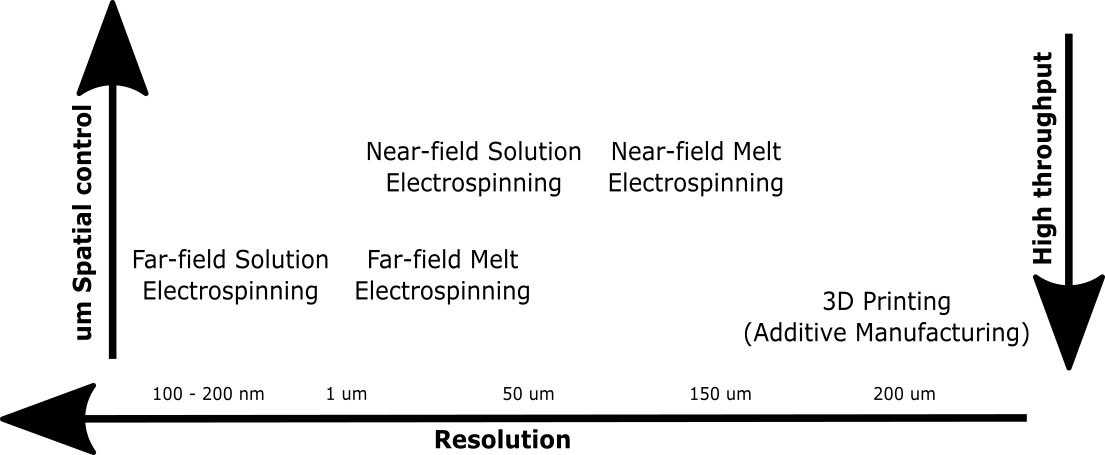
\includegraphics[scale=0.45]{./Figures/DifferentElectrospinningMethods.png}
\decoRule
\caption[Different Electrospinning Methods in Terms of Spatial Control, Fiber Throughput and Resolution]{Different Electrospinning Methods in Terms of Spatial Control, Fiber Throughput and Resolution. Adapted from \cite{Tourlomousis2017}}
\label{fig:DifferentElectrospinningMethods}
\end{figure}

As depicted in Figure \ref{fig:DifferentElectrospinningMethods}, solution electrospinning yields fibers with higher resolution than melt electrospinning techniques, and near-field electrospinning offers greater spatial control of the deposition of fibers than the far-field technique. Moreover, solution electrospinning often involves the use of toxic solvents, whereas melt electrospinning is a solvent free process but with the additional complexity as a heater needs to be installed. \cite{Tourlomousis2017}    
    
\section{Properties that Improve Accuracy of Nano-Fiber Deposition}
Near-field electrospinning is considered to be an outstanding technique to fabricate polymer fibers with spatial control and it has evolved through several modifications to improve the precision and accuracy of the fiber deposition. This work is intended to collect the NFES variants of electrospunable polymer solutions with spatial control in recent research. Appendix \ref{Appendix_NFESreviewTable} is a collection of the relevant NFES process parameters and achieved fiber morphology.

Some differences have been discovered between Low-Voltage Near-Field Electrospinning (LV-NFES) and conventional NFES. Low voltage near field electrospinning produces thinner fibers with lower voltages; as shown in Figure~\ref{fig:plt_Phi0V_vs_Dfiberm}. Moreover, when implementing a moving stage, the fibers are affected by the mechanical stretching. Bisht et al. and Chang et al. \unskip~\cite{527120:11973130,527120:11974313} reported that thinner diameters are obtained with the increase of the x-y stage velocity, and larger diameters by decreasing the stage velocity.

Bisht and Chang's work \unskip~\cite{527120:11973130,527120:11974313} reports a controlled technique to fabricate polymeric nano fibers in a continuous manner, using a low-voltage setup. Their purpose is to find a workaround to the drawbacks of traditional NFES by using a superelastic polymer precursor, which allows continuous patterning without breaking. In low voltage near-field electrospinning (LV NFES), a visco-elastic polymer is used to allow continuous spinning at about 200$V $.

Kim et al. \unskip~\cite{527120:11974313} experimented with a NFES variation where the fiber deposition is guided by conductive rails, see Figure~\ref{f-927e96fb5537}. As stated by the authors, the induced electric field is enhanced by the conductive pattern, which allows the fibers to follow the desired deposition path. As the fibers are prone to follow the conductive pattern, additional fibers can be stacked on top of the previously deposited fibers. The stacking process was successfully achieved in high electric field conditions at: 750$\mu m $ substrate to collector distance, and a 600 $\mu m $ needle to rail (offset) distance, see Figure~\ref{f-927e96fb5537}.


\bgroup
%\fixFloatSize{./images/0fd23deb-7631-4b09-8641-69fc6ac8a6b5-ukim_00.png}
\begin{figure*}[!htbp]
\centering \makeatletter\IfFileExists{./images/0fd23deb-7631-4b09-8641-69fc6ac8a6b5-ukim_00.png}{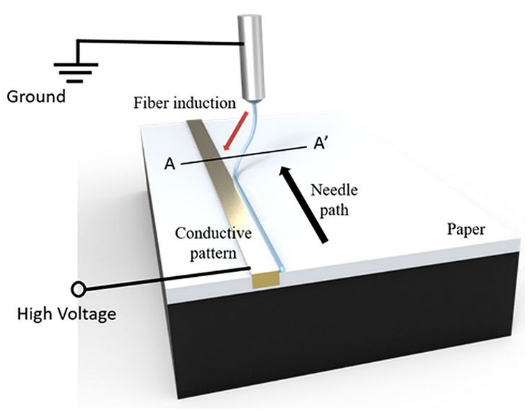
\includegraphics[scale=0.70]{./images/0fd23deb-7631-4b09-8641-69fc6ac8a6b5-ukim_00.png}}{}
\makeatother 
\caption{{NFES setup for controlled fiber deposition on pre-patterned conductive electrodes. Adapted from \unskip~\protect\cite{527120:11974313}}}
\label{f-927e96fb5537}
\end{figure*}
\egroup
Gupta et al.\unskip~\cite{527120:11974310} introduced a new technique to fabricate polymer scaffolds for tissue engineering applications and organ development. As described by Gupta et al.\unskip~\cite{527120:11974310}, the fiber deposition equipment is comprised by a stainless steel needle with a internal diameter of 750 $\mu m $ , connected to a high voltage power supply of up to 30 $k V $ with a deposition rate of about $\geq 1 \mu L min^{-1} $. The setup was embedded to a motorized collector capable of controlled programmable motions
%, see Figure~\ref{f-74de1f00848b}.
The proposed technique was able to produce fibers of $150 \mu m $ in diameter with pre-designed patterns.


\bgroup
%\fixFloatSize{./images/fa274bb7-a79d-48ae-9349-953df62c0094-ugupta_00.png}
%\begin{figure}[!htbp]
%\centering \makeatletter\IfFileExists{./images/fa274bb7-a79d-48ae-9349-953df62c0094-ugupta_00.png}{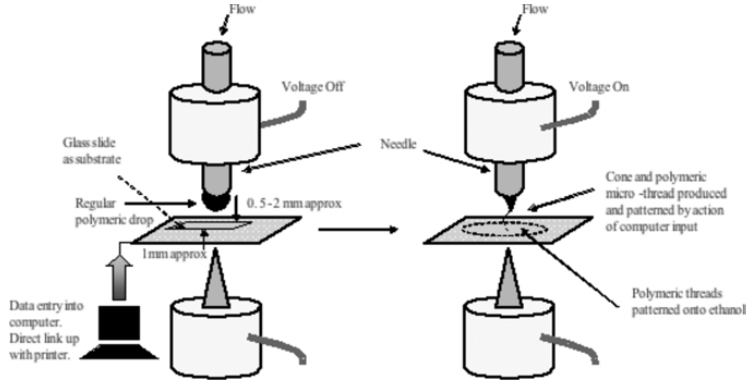
\includegraphics[scale=0.60]{./images/fa274bb7-a79d-48ae-9349-953df62c0094-ugupta_00.png}}{}
%\makeatother 
%\caption{{Schematic illustration of the electrohydrodynamic process. \unskip~\protect\cite{527120:11974310}}}
%\label{f-74de1f00848b}
%\end{figure}
\egroup
Wang, et al., Huang, et al., and Chen, et al. \unskip~\cite{527120:11974322,527120:11974323,527120:11974324} experimented with several multi-nozzle near-field electrospinning of aligned nano fibers. The multi-nozzle NFES apparatus is similar to the one used in conventional NFES with some modifications to the needle, see Figure \ref{f-4a1a1f58a423}. The authors implemented similar NFES setups where the installed linear array of nozzles is supplied with a constant flow rate of solution.

\bgroup
%\fixFloatSize{./images/cd8e0617-d4d9-479b-a99b-a466cd21483c-uwang_01.png}
\begin{figure}[!htbp]
\centering \makeatletter\IfFileExists{./images/cd8e0617-d4d9-479b-a99b-a466cd21483c-uwang_01.png}{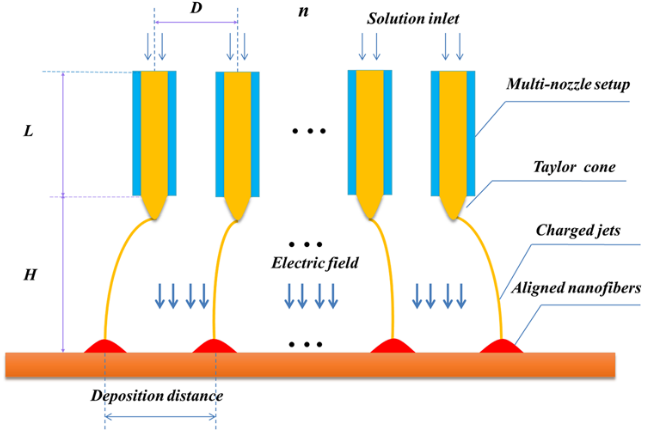
\includegraphics[scale=0.70]{./images/cd8e0617-d4d9-479b-a99b-a466cd21483c-uwang_01.png}}{}
\makeatother 
\caption[Geometry Distribution of Linear Array Multi-Nozzle System]{The geometry distribution of linear array multi-nozzle system. \unskip~\protect Adapted from \cite{527120:11974323}.}
\label{f-4a1a1f58a423}
\end{figure}
\egroup
The authors came to the conclusion that the distance between the deposited fibers increased as the needle-to-collector distance increased, due to the influence of the applied voltage dissipates.

Huang, et al.\unskip~\cite{527120:11974311} studied the mechanoelectrospinning (MES) technique for the fabrication of nano-fibers. The MES technique tries to improve deposition accuracy by the introduction of a mechanical drawing force. The MES is predominantly controlled by the collector stage velocity, the nozzle-to-collector distance, and the applied voltage. The authors believe that MES can compete as a low-cost, high precision fabrication of electronics and enable the direct writing of structures for nano-scale lithography. Figure~\ref{f-7587d8081ccc} shows the polymer jet behavior when a mechanical force is implemented within the NFES process.


\bgroup
%\fixFloatSize{./images/db7d3b35-fe08-422f-afe4-78e0133b489b-uhuang_00.png}
\begin{figure}[!htbp]
\centering \makeatletter\IfFileExists{./images/db7d3b35-fe08-422f-afe4-78e0133b489b-uhuang_00.png}{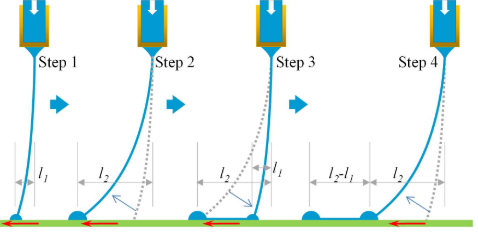
\includegraphics[scale=0.90]{./images/db7d3b35-fe08-422f-afe4-78e0133b489b-uhuang_00.png}}{}
\makeatother 
\caption[Schematic diagram of leap direct-writing]{Schematic diagram of leap direct-writing. Adapted from \cite{527120:11974311}}
\label{f-7587d8081ccc}
\end{figure}
% At a critical distance, the ink leaps to the next contact point, and gets stretched again \unskip~\protect\cite{527120:11974311}

\egroup
Micro and nano-fibers have been written using AC pulse-modulated electrospinning by Bu et al. with polyethylene terephthalate (PET) as substrate\unskip~\cite{527120:11974304}. The AC electrical field influences the electrospinning jet. The alternate current tends to decrease the repulsive electrical force allowing a stable straight jet between the dispensing nozzle and the insulating PET substrate. Bu et al. varied the stage velocity; faster stage velocities enable the deposition of straighter fibers\unskip~\cite{527120:11974304}.

 A mechano-electrospinning technique was presented by Nagle et al.\unskip~\cite{527120:12033656}. With the implementation of a mechanical drawing force, a higher resolution nano fibrous pattern can be produced with lower voltages as the Taylor cone becomes more stable. Nagle et al. studied PEO fibers at different nozzle-to-collector distances. Evidence suggests that better patterning accuracy increases with increasing nozzle to collector distance as the solution is effectively dried\unskip~\cite{527120:12033656}. Near field mechano-electrospinning enables the collection of non-woven fibers over large areas.


\bgroup
%\fixFloatSize{./images/43f61edd-73cd-4222-830e-3333f92934e9-uimg_nfesvariants.png}
\begin{figure}[!htbp]
\centering \makeatletter\IfFileExists{./images/43f61edd-73cd-4222-830e-3333f92934e9-uimg_nfesvariants.png}{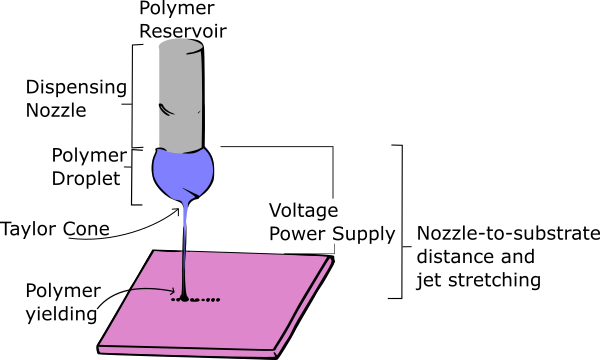
\includegraphics[scale=0.65]{./images/43f61edd-73cd-4222-830e-3333f92934e9-uimg_nfesvariants.png}}{}
\makeatother 
\caption{{Near-Field ES Process Parameters}}
\label{f-3629d3a3f9cf}
\end{figure}
\egroup
To spin nano-fibers at close distances, the initial diameter of the jet is required to be as small as possible since stretching of the thread is limited. Kameoka et al.\unskip~\cite{527120:12321556} demonstrated that a small initial spinning radius can be achieved using an atomic force microscope tip with a small polymer solution drop at the tip.

Near-field electrospinning, has been shown to enable the fabrication of nano-fibers and nano-fibrous patterns \unskip~\cite{527120:11974321}. Nevertheless, having a small polymer solution drop at the nozzle tip limits the length of the fibers that can be fabricated in a continuous manner. Using a spinneret with a reservoir (e.g. syringe) of solution generally produces fibers with diameter of a few micrometers \unskip~\cite{527120:11974310,527120:11974326}, since it creates a limit to which the nozzle inner diameter can be reduced to allow the solution to flow through. The implementation of thicker needle nozzles translates into an increase in diameter of the deposited polymer fibers.

Coppola et al.\unskip~\cite{527120:11974307} have showed a NFES variant that allows polymer nano-fibers to be deposited directly from a polymer drop, averting the issue of nozzle clogging. The fibers are also prone to soaking after deposition thus giving the fibers a semi-circular cross-section as shown by Xue and coworkers \unskip~\cite{527120:11974326}.



\subsection{Nozzle spinneret}The thinnest nozzles in literature so far are about $50 \textrm{ nm}$ in diameter, by Chang et al.\unskip~\cite{527120:11974306} who used a  $100 \textrm{ } \mu \textrm{m}$ inner diameter needle tip to electrospin poly(ethylene oxide) (PEO). Camillo et al.\unskip~\cite{527120:12322072} used a micro-diameter-tip Tungsten spinneret in a 26G needle to electrospin co-polymer, poly[2-methoxy-5-(2-ethylhexyloxy)-1,4-phenylenevinylene] (MEH-PPV) with poly(ethylene oxide) (PEO). The nozzle most commonly comprises a simple narrow-bore, blunt-end metal needle. The diameter of the needle can vary, but most commonly researches work with internal diameters below 1 $mm $ . This translates to needles of gauge 18{\textendash}22. In general, this simple spinneret design can be used to achieve successful spinning. A blunt-end rather than a tapered-end for the needle exit is important as the size distribution of the products increase with an increase in needle tip angle. However, it should be noted that there will be some interactions between the solvent and polymer molecules in the solution and the metal surface of the spinneret. There will exist some attractive forces between the polar groups in the polymer and the electro-positive metal surface, which can act counter to the drawing force of the electric field and can pull the polymer solution back into the spinneret. It has been found that coating the spinneret exterior in a non-conductive and non-stick polymer such as Teflon or epoxy coating can reduce these interactions.\unskip~\cite{527120:13082768,527120:13082811} As a result, the electrical energy can be more efficiently used to elongate and narrow the polymer jet, and narrower fibers can be produced. In addition, strong attractive forces between the polymer jet and the metal spinneret can result in fibers becoming attracted to the needle, leading to lower yields and potentially to blocking of the exit orifice.



\subsection{Applied Voltage}In recent literature, near field electrospinning has been studied to reduce the fiber diameter and to improve the control over fiber deposition. Madou et al.\unskip~\cite{527120:11973130} and Chang et al.\unskip~\cite{527120:11974306} came to the conclusion that higher voltages yield thicker micro-fibers with a loss in jet stability. This relationship between the applied voltage and resulting fiber diameter is influenced by other variables such as nozzle-to-substrate distance and solution deposition rate. For instance, if a high voltage is applied at a low deposition rate then electrospraying is achieved, meaning the formation of several non-continuous fibers. The applied voltage shall be sufficient to break the surface tension and initiate the jet, but low enough to avoid multiple jets at the nozzle tip.

Madou et al.\unskip~\cite{527120:11973130} achieved the fabrication of thinner fibers with spatial control by reducing the applied voltage to 200-600 $V $  at a nozzle-to-substrate distance of 0.5-1 $mm $. The low voltage setting alone does not create enough charge to break the polymer solution surface tension to initiate the electrospinning process. Madou et al.\unskip~\cite{527120:11973130} and Chang et al.\unskip~\cite{527120:11974306} initiated the electrospun fibers by mechanically pulling the polymer solution at the nozzle tip using a micro-probe tip. Chang and coworkers reduced the applied voltage from 1.5 $kV $ to 600 $V $ with a nozzle-to-substrate distance of 500 $\mu m $ to yield a fiber diameter between 3 $\mu m $  and 50 $nm $ . With an applied voltage of 200 $V $ and a nozzle-to-substrate distance of 1 $mm $.

In near-field electrospinning, the applied voltage has an impact on the morphology of the fiber. For instance, a voltage higher or lower to the optimum voltage will translate into an increase in fiber diameter. Song et al.\unskip~\cite{527120:11974320} demonstrated that an increase in voltage from 400 to 500 $V $ can reduce the fiber diameter from 160 to about 60 $nm $with a nozzle-to-substrate distance of 20 $\mu m $. A workaround to break the polymer solution surface tension is to initialize the NFES process with a higher voltage and then lower the voltage once the jet is created. Huang et al.\unskip~\cite{527120:11974311} implemented the previous and obtained ordered fibers with a distance between adjacent fibers of 50 $\mu m $.

\subsection{Nozzle-to-substrate distance}
\bgroup
%\fixFloatSize{./images/4cc65220-1457-4d0d-bb04-9b1c8138aa96-uffes_vs_nfes.png}
\begin{figure*}[!htbp]
\centering \makeatletter\IfFileExists{./images/4cc65220-1457-4d0d-bb04-9b1c8138aa96-uffes_vs_nfes.png}{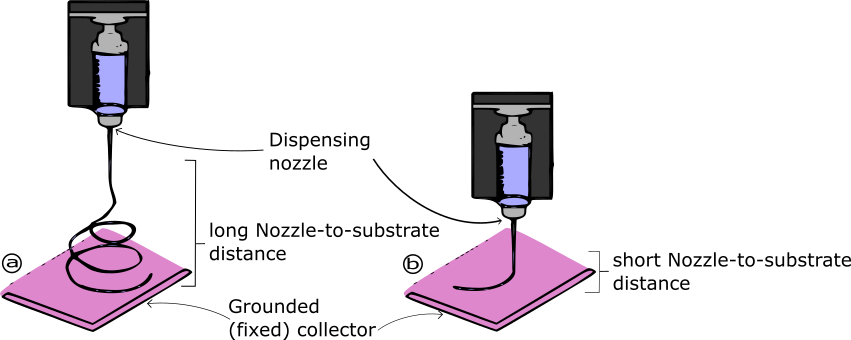
\includegraphics[scale=0.65]{./images/4cc65220-1457-4d0d-bb04-9b1c8138aa96-uffes_vs_nfes.png}}{}
\makeatother 
\caption{{a) Typical Far-field Electrospinning (FFES) Setup. b) Typical Near-field Electrospinning (NFES) Setup.}}
\label{f-c34559531e3e}
\end{figure*}
\egroup
Figure~\ref{f-c34559531e3e}.a, depicts the typical setup for the conventional far-field electrospinning (FFES). As stated in previous sections, the precursor polymer droplet becomes charged with the employment of an electric field between the polymer solution and the collector\unskip~\cite{527120:14135125}. When the polymer solution surface tension is overcome by the electric field potential difference, a jet is formed, starting the electrospinning process. The electrospinning process can be broken down into two steps: i) first the jet travels in a straight line, and ii) the jet begins to curl due to bending and whipping instabilities \unskip~\cite{527120:13444381,527120:14135543}. The fiber spatial control in far-field electrospinning is limited due to the instabilities, inhibiting the precise deposition of fibers.

With the goal of achieving controlled fiber deposition, Sun et al. \unskip~\cite{527120:11974321} reported an electrospinning variation known as near-field electrospinning (NFES),Figure~\ref{f-c34559531e3e}.b, describes the near-field electrospinning setup, where the distance between the dispensing nozzle and the collector is reduced to write fibers while the jet travels in a straight line. Moreover, some mechanical influence is required to deposit fibers with higher precision. The mechanical force is introduced by moving collector. If the polymer solution jet speed is faster than the speed of the moving collector, the written fiber will curl; on the other hand, if the collector moves faster than the polymer jet, the fiber will gradually diminish \unskip~\cite{527120:11974327,527120:11974326}. Currently, due to the lack of theoretical models, the near-field electrospinning process parameters (such as the collector speed) are typically tuned by experience and experimentation only. Adimensional analyses have been done \cite{Sarkar2009,Tourlomousis2017,Cai2013,Wang2008a,Widartiningsih2020,Chang2014,Brooks2015,Helgeson2008,Helgeson2007,Gadkari2014} and can be used as a guide to design and prepare electrospinning setups, however these analyses are recently developed and hence their little appearance in literature publications.

The main difference between NFES and FFES is the distance between the needle and the collector which is higher in FFES (about 10 cm) compared to NFES, which ranges in the mm scale. The short distance allows the production of well-aligned fibers within particular designs. In NFES, the fiber morphology can be altered by the control of the distance between the nozzle and the substrate (collector). With the decrease of the nozzle-to-substrate distance, the electric field strength increases; however it can cause incomplete solvent volatilisation and possible short circuits between the collector and the nozzle tip.

An optimal nozzle-to-substrate distance shall be defined to ensure the fabrication of dry continuous fibers. If the solvent is not well evaporated, the produced fibers are prone to defects; on the other hand, if solidification happens too fast, the solids can block the spinneret which can prevent a continuous fiber yield. Furthermore, the polymer jet will discharge itself as soon as possible, therefore long distances can result in low yields.

\subsection{Substrate}Due to the close distance between the grounded substrate and the charged spinneret in NFES, the set up is prone to electrical shorts. In NFES, when a short circuit takes place, the electrospinning process is interrupted resulting in the fabrication of discontinuous fibers. Two workarounds to avoid electrical shorts is to lower the applied voltage and to use less conductive substrates \unskip~\cite{527120:11974315,527120:12322289}.

Liu et al.\unskip~\cite{527120:11974315} discovered that the fiber alignment is improved by using a glass-cooper foil substrate, however the alignment of the fibers is spoiled after prolonged depositions due to residual charges. Additionally, the effect of residual charges is amplified when the used collector substrate contains a conductive layer and a non-conductive layer\unskip~\cite{527120:11974315}.

In contrast, Choi et al.\unskip~\cite{527120:12322289} implemented a hydrophilic substrate to deposit the fibers with plasma treatment to increase the conductivity of selected areas. NFES was carried out with precise deposition as the fibers were placed as per the desired design within the hydrophilic substrate.

\section{Data collection of NFES fiber morphology and process parameters}

The near-field electrospinning process parameters and the morphological data (diameters and images) reported in papers reviewed was collected and classified into a single database with the purpose of analyzing and finding correlations between the process parameters and the obtained fiber diameter after a NFES process. The analysis was based from data ranging from the first reported NFES apparatus built in 2003 by J. Kameoka et al. \cite{Kameoka2003a} to recent studies conducted in 2020. \cite{
  Yang2019,Fattahi2017,Shin2019,Wang2015,Parajuli2016,Zheng2010,Fuh2011,Dalton2015,
  Ru2014,Xue2014,Wang2017,Xu2014,Liu2013,Pan2014,Canton2014,Chakraborty2009,Gupta2007,
  He2018,Zhou2011,Chen2013,Williams2018,Choi2017,Pan2019,Lei2015,Lim2019,Park2020,
  Fuh2012,Flores2017,Chang2010,Xu2019,Zhang2019,Shin2018,Fuh2015,Nagle2019,Zheng2012,
  Kameoka2003a,Liu2014,E.King2019,Hochleitner2017,Madou2011,Jiang2018,Husain2016,
  ElectrospinTech2015,Brown2011,Kolan2018,Chang2011,Beachley2011,Camillo2013,Kameoka2003,
  Bu2012,Lee2012,Huang2015,Coppola2020,CisquellaSerra2019,Ruggieri2013,Hochleitner2014,
  Zhu2016,Brown2014,Chang2008,Sonntag2020,Kim2018,Deng2020,Han2019,George2020,Sun2006a,
  Pan2015,Shen2016,Strauss2019,Fuh2013,Sarkar2007,You2017,Wang2018a,Zheng2014,Song2015,
  GaofengZheng2010,Liu2015a,Min2013,Luo2016,Yousefi2019,Cardenas2017,Coppola2014} The data was divided in three groups depending on the format of the available information, as follows:

\begin{enumerate}
\item Case 1 : data is collected as-is from literature. This procedure was implemented when the data is listed within tables and/or as text format.
\item Case 2 : data is only presented in a figure as plots.
\item Case 3 : data is not available in text format or plots, however Scanning Electron Microscopy (SEM) images are reported from the obtained fibers.
\end{enumerate}

\subsection{Image Analysis - Data extraction from plots}

Most numerical data of NFES process parameters and fiber diameters is available only in the form of plots. The reported figures provide a visual relationship between the variables of interest, however recovering the numerical values of the data is a tedious process prone to errors. To avoid mistakes and accelerate the acquicition of data from the plots, \href{https://github.com/ankitrohatgi/WebPlotDigitizer}{WebPlotDigitizer} was used. WebPlotDigitizer is a HTML5 tool that facilitates accurate data extraction with ease of use. Figure \ref{fig:screenshotWebPlotDigitizer} is a screenshot of the software in use.

\begin{figure}[!th]
\centering
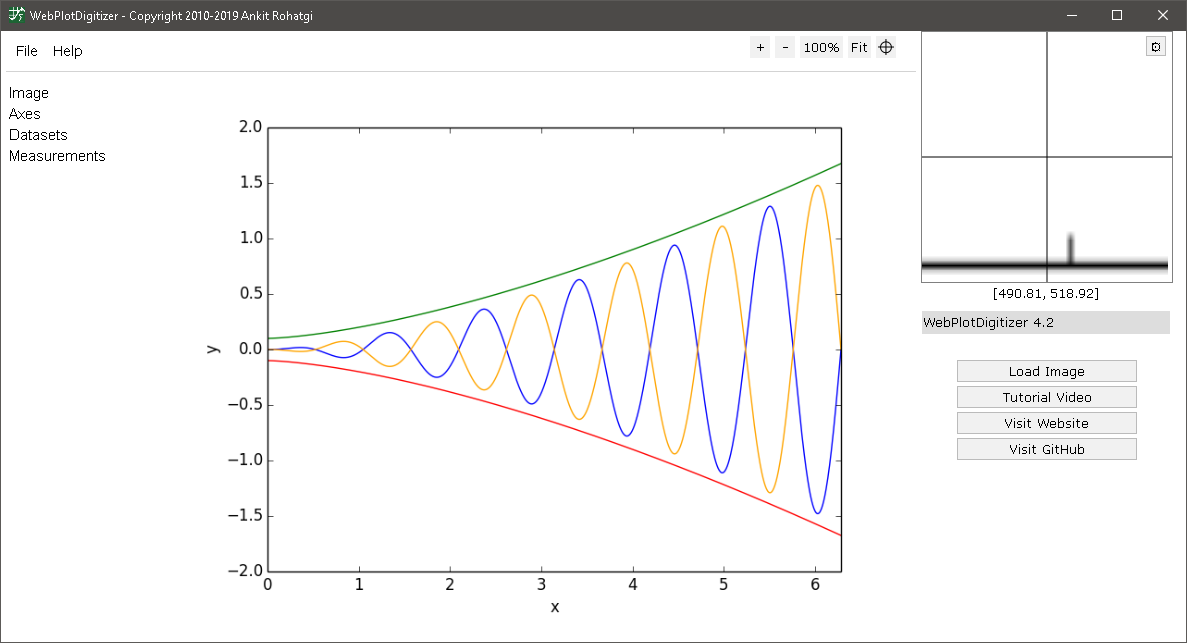
\includegraphics[scale=0.45]{./Figures/screenshotWebPlotDigitizer.png}
\decoRule
\caption[WebPlotDigitizer home-screen]{Open session of WebPlotDigitizer \href{https://github.com/ankitrohatgi/WebPlotDigitizer}{github.com}}
\label{fig:screenshotWebPlotDigitizer}
\end{figure}

\subsection{Image Analysis - Data extraction from Scanning Electron Microscopy Images}

Scanning Electron Microscopy Images (SEM) images contain information in a two-dimensional grid that can be extracted using point and line counting techniques, however this can be a laborious process for a large number of images. To decrease the complex and lavorious aspect of the counting process, a \emph{Python} script was developed to measure fiber diameters from the available SEM images. As shown in Figure \ref{fig:imageAnalysisAlgorithm}, the image analysis algorithm follows three main steps: pre-processing, segmentation, object detection, and data processing.

\begin{figure}[!th]
\centering
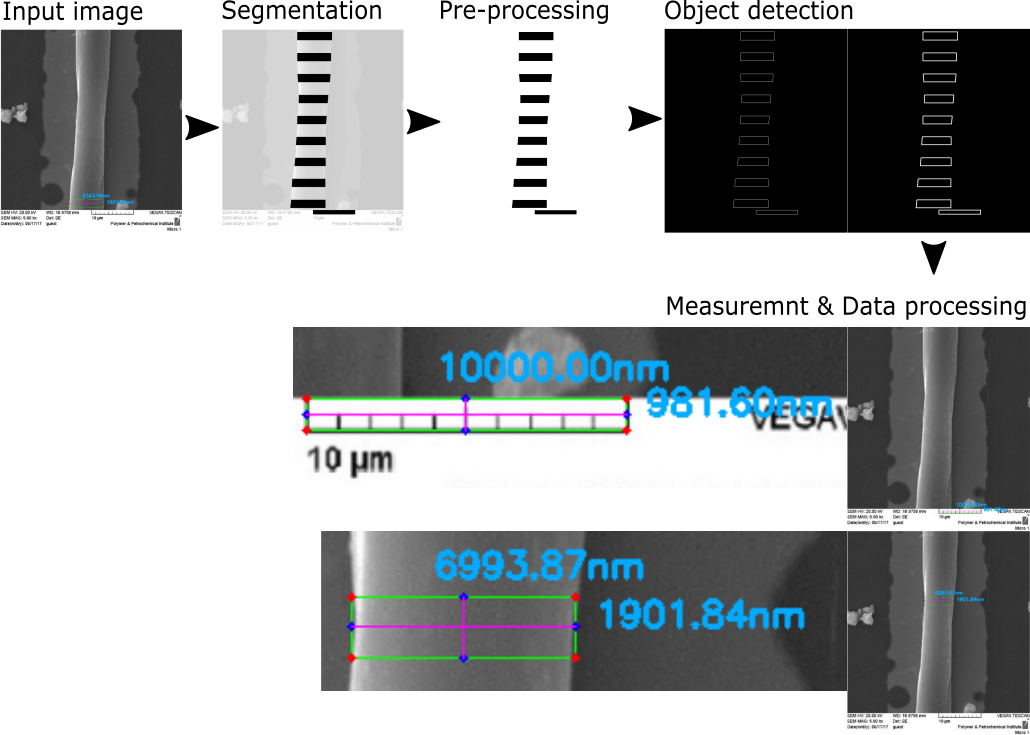
\includegraphics[scale=0.50]{./Figures/imageAnalysisAlgorithm.png}
\decoRule
\caption[Image Analysis Algorithm to Measure Fiber Diameters from SEM images]{Image Analysis Algorithm to Measure Fiber Diameters from SEM images. Ilustration uses Yousefi et al.'s work as an example. \cite{Yousefi2019}}
\label{fig:imageAnalysisAlgorithm}
\end{figure}

The adopted image analysis was implemented with the \emph{Python} package \emph{OpenCV} (Appendix \ref{Appendix_ImageAnalysisCode}). First a segmentation procedure is executed over an input image to delimit the objects to be measured (fiber sections and scale-bars). The segmentation step is the only step needed to be done manually in a image processing software, in this case \emph{Inkscape} was used. Next, the segmented image is passed into the \emph{Pyhton} script, which will convert its input image into a binary image. A binary image is a black and white image (with no gray scale) that facilitates the detection of the object edges as the color intensity change between the objects and the background is well-defined. Once the binary image is computed, the \emph{Canny} edge detection algorithm is executed. Once the edges are well-defined, the image is dilated to make the edges more visible. The final step before measurement, the \emph{OpenCV} \emph{findContours} function is called to store the objects in memory. The first object to be measured is the scale bar as this is needed as a reference to convert the pixel counts to a metric unit. Finally, the objects are located within the image with four edge points, and the reference object is used to compute the metric length as the ratio of counted pixels between two edge points and the scale bar dimension in meters.

Measurements were validaded with Camillo's, Gupta's, Jiang's, Min's, Sun's, Wang's, and Xue's \cite{Camillo2013, Gupta2007, Jiang2018, Min2013, Sun2006a, Wang2015, Xue2014} results as those authors reported both, a SEM image and the measured fiber diameter. For instance, Figure \ref{fig:imageAnalysisToolValidation} shows in black the reported diameters by Min and in white the diameters measured by the \emph{Python script} of two samples. The measurement error of the developed script is about $3.2\%$ in average. It is considerable to mention that the reported measurement error is mainly contributed to the fact that most fibers are not of the same diameter along the fiber length. In most cases, measurements at the end of the fibers are thicker than the ones measured in the center.

\begin{figure}[!th]
\centering
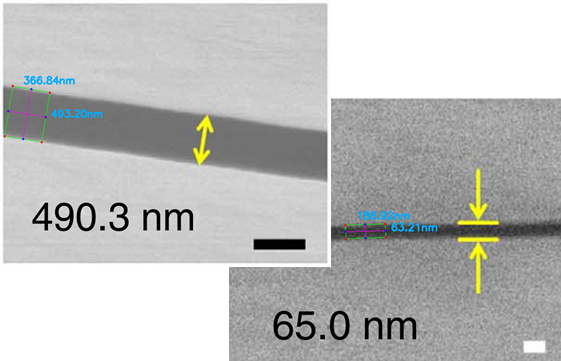
\includegraphics[scale=0.8]{./Figures/imageAnalysisToolValidation.png}
\decoRule
\caption[Validation of the developed image analysis meassurement tool]{{Validation of the developed image analysis meassurement tool. SEM images of Min's work are used as an example. \cite{Min2013}}}
\label{fig:imageAnalysisToolValidation}
\end{figure}

\section{Discussion \& NFES Challenges}
\label{sec:parametersThatAffectTheDiameter}

Helix electrodynamic printing (HE-printing) was presented by Duan et al. \unskip~\cite{527120:11974308} with the intention of depositing aligned fibers. The authors fabricated a stretchable piezoelectric device using micro- and nano-fibers to demonstrate the possible applications of HE-printing for electronics manufacturing. Duan et al. concluded that the fiber morphology is mainly affected by: the stage velocity, the applied voltage, and the nozzle-to-collector distance.

\begin{figure}[!th]
\centering
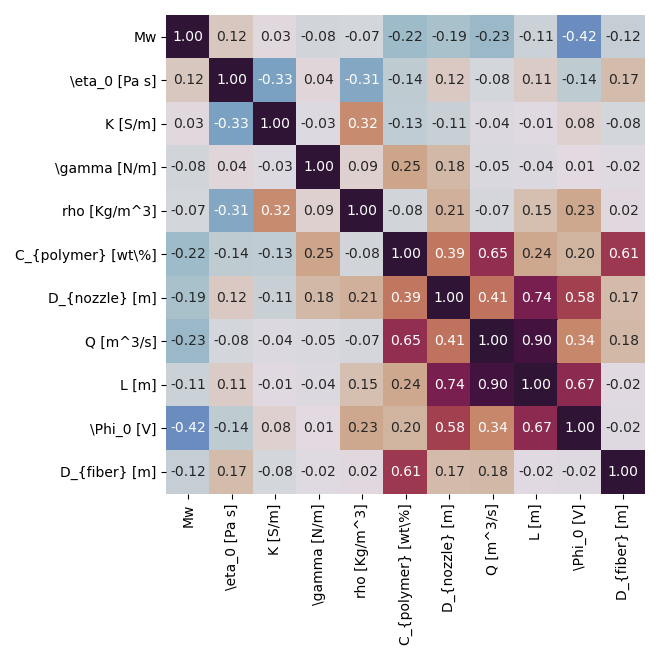
\includegraphics[width=\textwidth]{./Figures/plt_corMat.png}
\decoRule
\caption[NFES correlation matrix of process parameters and fiber morphology]{{Correlation matrix comprised by the NFES data from recent literature. 
\cite{
  Yang2019,Fattahi2017,Shin2019,Wang2015,Parajuli2016,Zheng2010,Fuh2011,Dalton2015,
  Ru2014,Xue2014,Wang2017,Xu2014,Liu2013,Pan2014,Canton2014,Chakraborty2009,Gupta2007,
  He2018,Zhou2011,Chen2013,Williams2018,Choi2017,Pan2019,Lei2015,Lim2019,Park2020,
  Fuh2012,Flores2017,Chang2010,Xu2019,Zhang2019,Shin2018,Fuh2015,Nagle2019,Zheng2012,
  Kameoka2003a,Liu2014,E.King2019,Hochleitner2017,Madou2011,Jiang2018,Husain2016,
  ElectrospinTech2015,Brown2011,Kolan2018,Chang2011,Beachley2011,Camillo2013,Kameoka2003,
  Bu2012,Lee2012,Huang2015,Coppola2020,CisquellaSerra2019,Ruggieri2013,Hochleitner2014,
  Zhu2016,Brown2014,Chang2008,Sonntag2020,Kim2018,Deng2020,Han2019,George2020,Sun2006a,
  Pan2015,Shen2016,Strauss2019,Fuh2013,Sarkar2007,You2017,Wang2018a,Zheng2014,Song2015,
  GaofengZheng2010,Liu2015a,Min2013,Luo2016,Yousefi2019,Cardenas2017,Coppola2014} Fiber diameter is highly correlated with polymer solution concentration and slightly correlated with solution flow rate, zero-shear viscosity and nozzle diameter.}}
\label{fig:plt_corMat}
\end{figure}

Figures \ref{fig:plt_Cpolymerwt_vs_Dfiberm}, \ref{fig:plt_Dnozzlem_vs_Dfiberm}, \ref{fig:plt_Lm_vs_Dfiberm}, \ref{fig:plt_Phi0V_vs_Dfiberm}, \ref{fig:plt_Qm3s_vs_Dfiberm} and \ref{fig:plt_vstagems_vs_Dfiberm} are scatter plots that depict the relationship of various process parameters (polymer concentration $C_{polymer}$, nozzle inner diameter $D_{nozzle}$, NFES working distance $L$, NFES applied voltage $\Phi_0$, flow rate $Q$, and stage velocity $v_{stage}$) with the final fiber diameter $D_{fiber}$. In a generalized summary, these figures suggest that thin fibers are produced with the implementation of low polymer concentrations, small nozzle diameters, short working distances, low applied voltages, low flow rates, and high stage xy velocities. Moreover, based on the degree of dispersion of the data points, polymer concentration $C_{polymer}$ is the most reliable process parameter to describe and predict the behavior of the fiber diameter, as most of the data can be grouped in a single cluster. Unlike $C_{polymer}$ in Figure \ref{fig:plt_Cpolymerwt_vs_Dfiberm}, various data clusters can be identified within the other scatter plots. For instance, Song's results \cite{Song2015} deviate from the main cluster in Figures \ref{fig:plt_Dnozzlem_vs_Dfiberm}, \ref{fig:plt_Lm_vs_Dfiberm}, \ref{fig:plt_Phi0V_vs_Dfiberm}, and \ref{fig:plt_vstagems_vs_Dfiberm}, this may be because Song et al. used Au/Pd coated glass capillary nozzles instead of the traditional stainless steel precision tips. However in the $C_{polymer}$ vs. $D_{fiber}$ figure, Song's results fit within the main cluster.

\begin{figure}[!th]
\centering
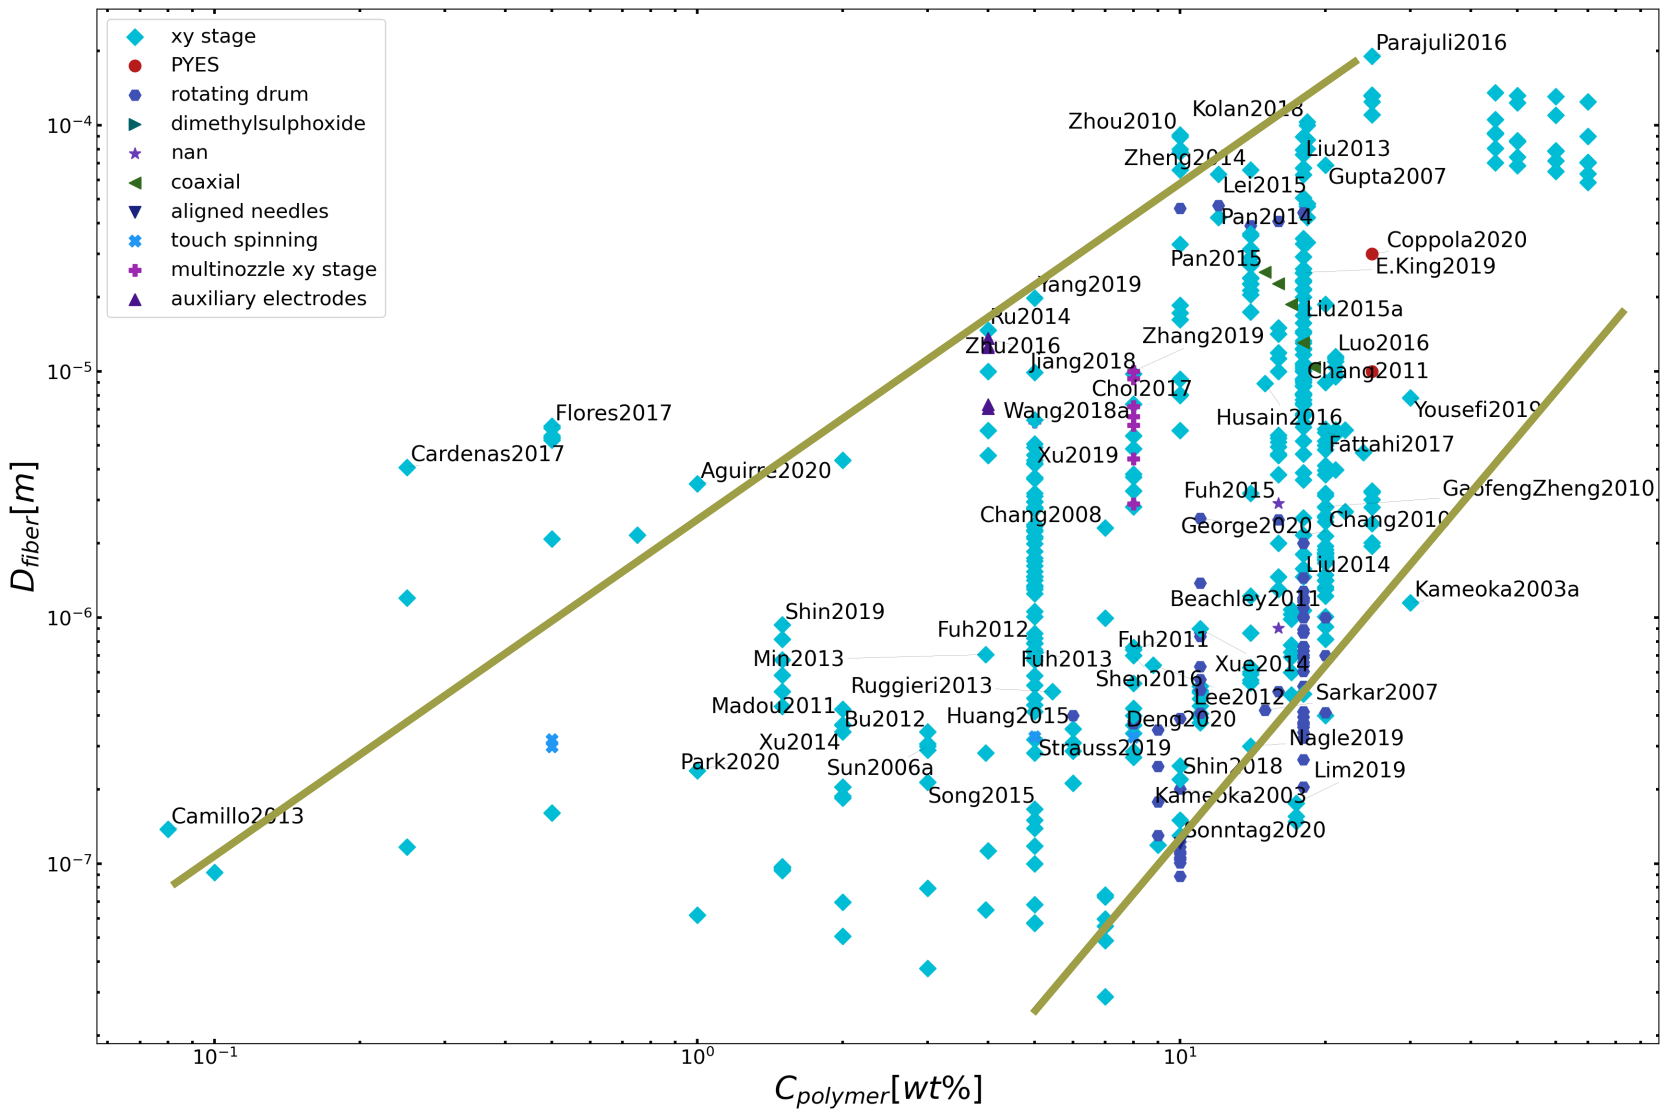
\includegraphics[width=\textwidth]{./Figures/plt_Cpolymerwt_vs_Dfiberm.png}
\decoRule
\caption[Scatter Plot of Polymer Concentrations and Fiber Diameters from Literature Experimental Results]{Scatter Plot of Polymer Concentrations and Fiber Diameters from Literature Experimental Results. \cite{
  Yang2019,Fattahi2017,Shin2019,Wang2015,Parajuli2016,Zheng2010,Fuh2011,Dalton2015,
  Ru2014,Xue2014,Wang2017,Xu2014,Liu2013,Pan2014,Canton2014,Chakraborty2009,Gupta2007,
  He2018,Zhou2011,Chen2013,Williams2018,Choi2017,Pan2019,Lei2015,Lim2019,Park2020,
  Fuh2012,Flores2017,Chang2010,Xu2019,Zhang2019,Shin2018,Fuh2015,Nagle2019,Zheng2012,
  Kameoka2003a,Liu2014,E.King2019,Hochleitner2017,Madou2011,Jiang2018,Husain2016,
  ElectrospinTech2015,Brown2011,Kolan2018,Chang2011,Beachley2011,Camillo2013,Kameoka2003,
  Bu2012,Lee2012,Huang2015,Coppola2020,CisquellaSerra2019,Ruggieri2013,Hochleitner2014,
  Zhu2016,Brown2014,Chang2008,Sonntag2020,Kim2018,Deng2020,Han2019,George2020,Sun2006a,
  Pan2015,Shen2016,Strauss2019,Fuh2013,Sarkar2007,You2017,Wang2018a,Zheng2014,Song2015,
  GaofengZheng2010,Liu2015a,Min2013,Luo2016,Yousefi2019,Cardenas2017,Coppola2014}}
\label{fig:plt_Cpolymerwt_vs_Dfiberm}
\end{figure}

The trend of Figure \ref{fig:plt_Dnozzlem_vs_Dfiberm} shows that thicker nozzle diameters yield thicker fibers. However, the final fiber diameter can be reduced without changing the nozzle diameter. For instance Chang et al. \cite{Chang2008} achieved the thinnest fibers of about $50 \textrm{ nm}$ in diameter even though Chang implemented nozzle needles of similar diameter as Shin, Min and Xu by the implementation of different settings on the other process parameters. For instance: the glass glass capillary nozzles by Song \cite{Song2015}, the melt-NFES setup by \cite{Brown2011, Brown2014}, the long working distances implemented by Husain \cite{Husain2016}, the low stage velocities by Shin \cite{Shin2019} to fabricate coiled fibers, and the high polymer concentrations by Parajuli \cite{Parajuli2016} are some differences from the traditional NFES setup that are represented as isolated clusters within Figures \ref{fig:plt_Cpolymerwt_vs_Dfiberm}, \ref{fig:plt_Dnozzlem_vs_Dfiberm}, \ref{fig:plt_Lm_vs_Dfiberm}, \ref{fig:plt_Phi0V_vs_Dfiberm}, \ref{fig:plt_Qm3s_vs_Dfiberm} and \ref{fig:plt_vstagems_vs_Dfiberm}. It is worth nothing that Chang's thinnest fiber may be a one-time result where, neither the yield rate nor the reproducibility of their technique was not reported.

\begin{figure}[!th]
\centering
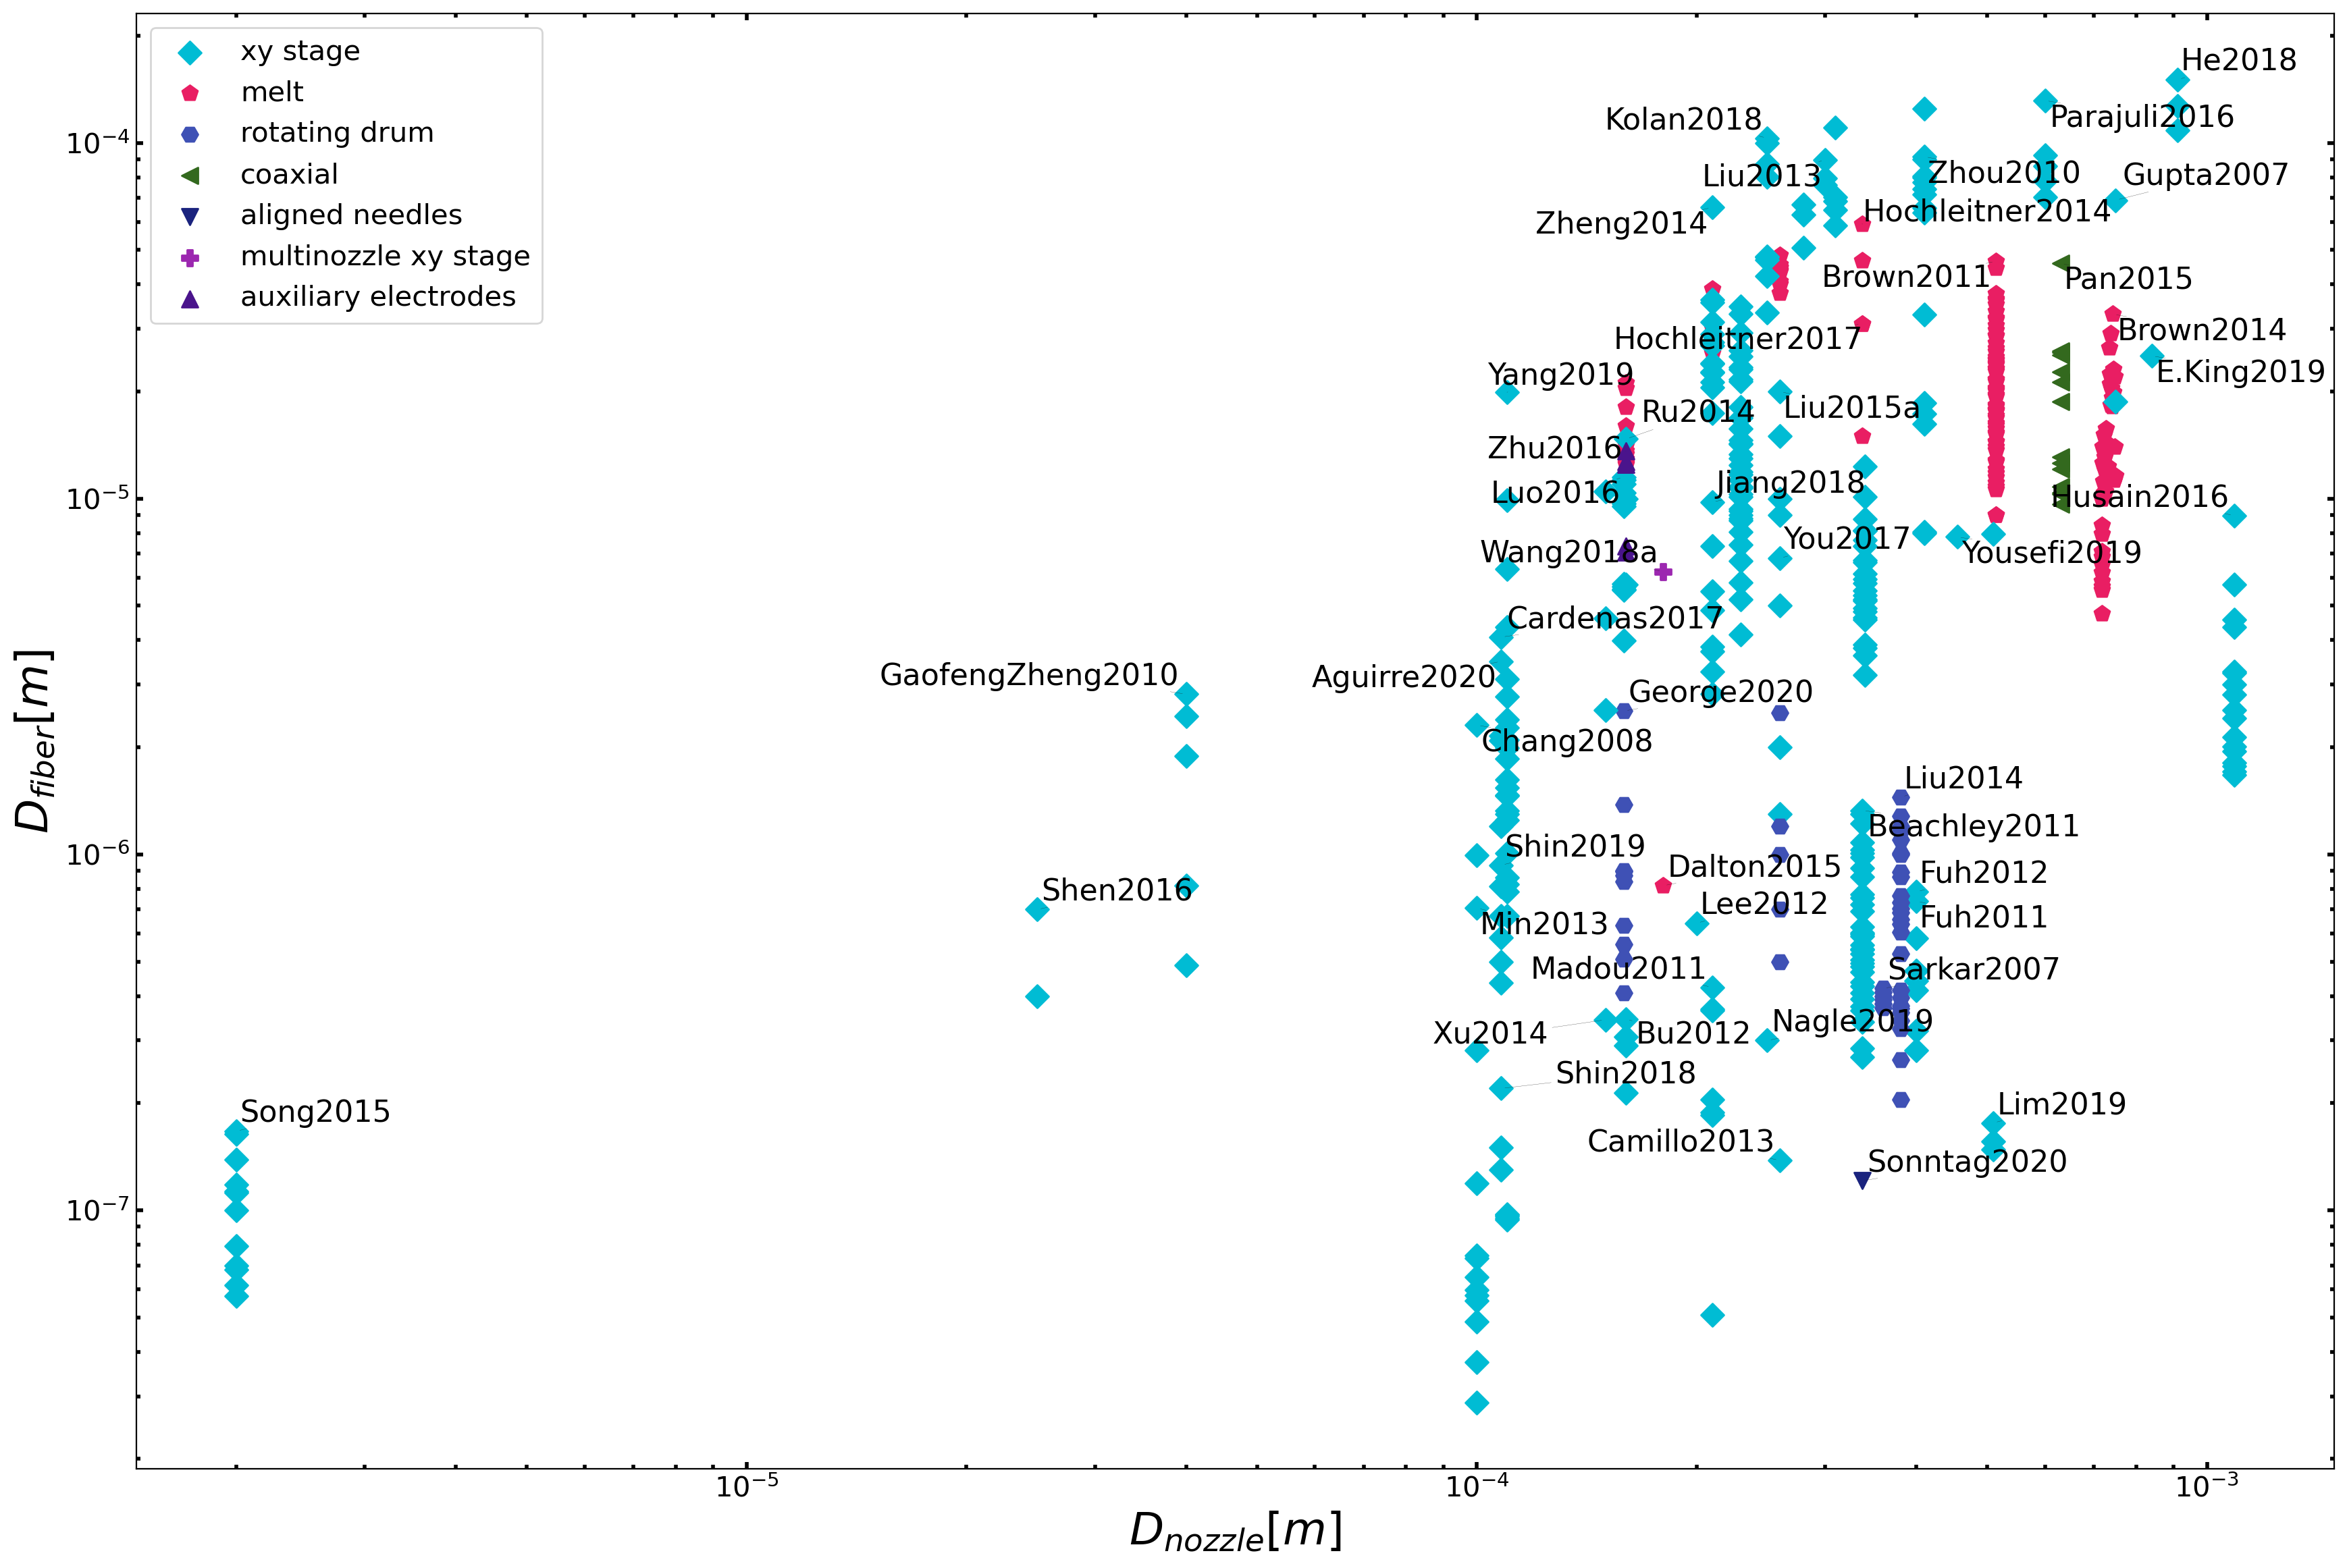
\includegraphics[width=\textwidth]{./Figures/plt_Dnozzlem_vs_Dfiberm.png}
\decoRule
\caption[Scatter Plot of Nozzle Inner Diameters and Fiber Diameters from Literature Experimental Results]{Scatter Plot of Nozzle Inner Diameters and Fiber Diameters from Literature Experimental Results. \cite{
  Yang2019,Fattahi2017,Shin2019,Wang2015,Parajuli2016,Zheng2010,Fuh2011,Dalton2015,
  Ru2014,Xue2014,Wang2017,Xu2014,Liu2013,Pan2014,Canton2014,Chakraborty2009,Gupta2007,
  He2018,Zhou2011,Chen2013,Williams2018,Choi2017,Pan2019,Lei2015,Lim2019,Park2020,
  Fuh2012,Flores2017,Chang2010,Xu2019,Zhang2019,Shin2018,Fuh2015,Nagle2019,Zheng2012,
  Kameoka2003a,Liu2014,E.King2019,Hochleitner2017,Madou2011,Jiang2018,Husain2016,
  ElectrospinTech2015,Brown2011,Kolan2018,Chang2011,Beachley2011,Camillo2013,Kameoka2003,
  Bu2012,Lee2012,Huang2015,Coppola2020,CisquellaSerra2019,Ruggieri2013,Hochleitner2014,
  Zhu2016,Brown2014,Chang2008,Sonntag2020,Kim2018,Deng2020,Han2019,George2020,Sun2006a,
  Pan2015,Shen2016,Strauss2019,Fuh2013,Sarkar2007,You2017,Wang2018a,Zheng2014,Song2015,
  GaofengZheng2010,Liu2015a,Min2013,Luo2016,Yousefi2019,Cardenas2017,Coppola2014}}
\label{fig:plt_Dnozzlem_vs_Dfiberm}
\end{figure}

The relationship between the fiber diameter, the working distance $L$ and applied voltage $\Phi_0$ can be depicted in Figures \ref{fig:plt_Lm_vs_Dfiberm} and \ref{fig:plt_Phi0V_vs_Dfiberm}. The near-field electrospinning jet is ejected from the Taylor cone when the applied voltage generates an electric field strong enough to break the solution drop. Changing the applied voltage will change initial drop shape, thereby resulting in a change in the fibers' diameters. However, the effect of the applied voltage on the fiber diameter is not well understood. On one hand, many researchers posit that high applied voltages lead to larger fiber diameters, whereas other researchers have reported reductions in fiber diameter with high applied voltages as the electric field force increases on the charged jet. \cite{Zhang2005} Furthermore, Reneker and Chun observed that applied voltage does not significantly affect the diameter of electrospun polyethylene oxide (PEO) fibers. \cite{Reneker1996} Applied voltage has an influence on the fiber diameter, but the degree and direction of the effect on the diameter varies with other process parameters such as polymeric solution concentration and on the working distance \cite{Yordem2008, Chang2016}.

Looking at Figures \ref{fig:plt_Lm_vs_Dfiberm} and \ref{fig:plt_Phi0V_vs_Dfiberm}, the data points from Husain, Lee and Sonntag \cite{Husain2016, Lee2012, Sonntag2020} are outside the principal cluster since they implemented working distances around $10^{-1} \textrm{m}$, which is considered to be the threshold between NFES and far-field electrospinning (FFES). One can observe that: a) in NFES fiber diameter increase with increasing applied voltage; and b) in FFES fiber diameter decrease with increasing applied voltage. On the other hand, data related to Liu's and Beachey's work \cite{Liu2014, Beachley2011} do not fit the main trend as they performed the electrospinning process with a rotating drum as the collector, instead of the typical xy stage. 

\begin{figure}[!th]
\centering
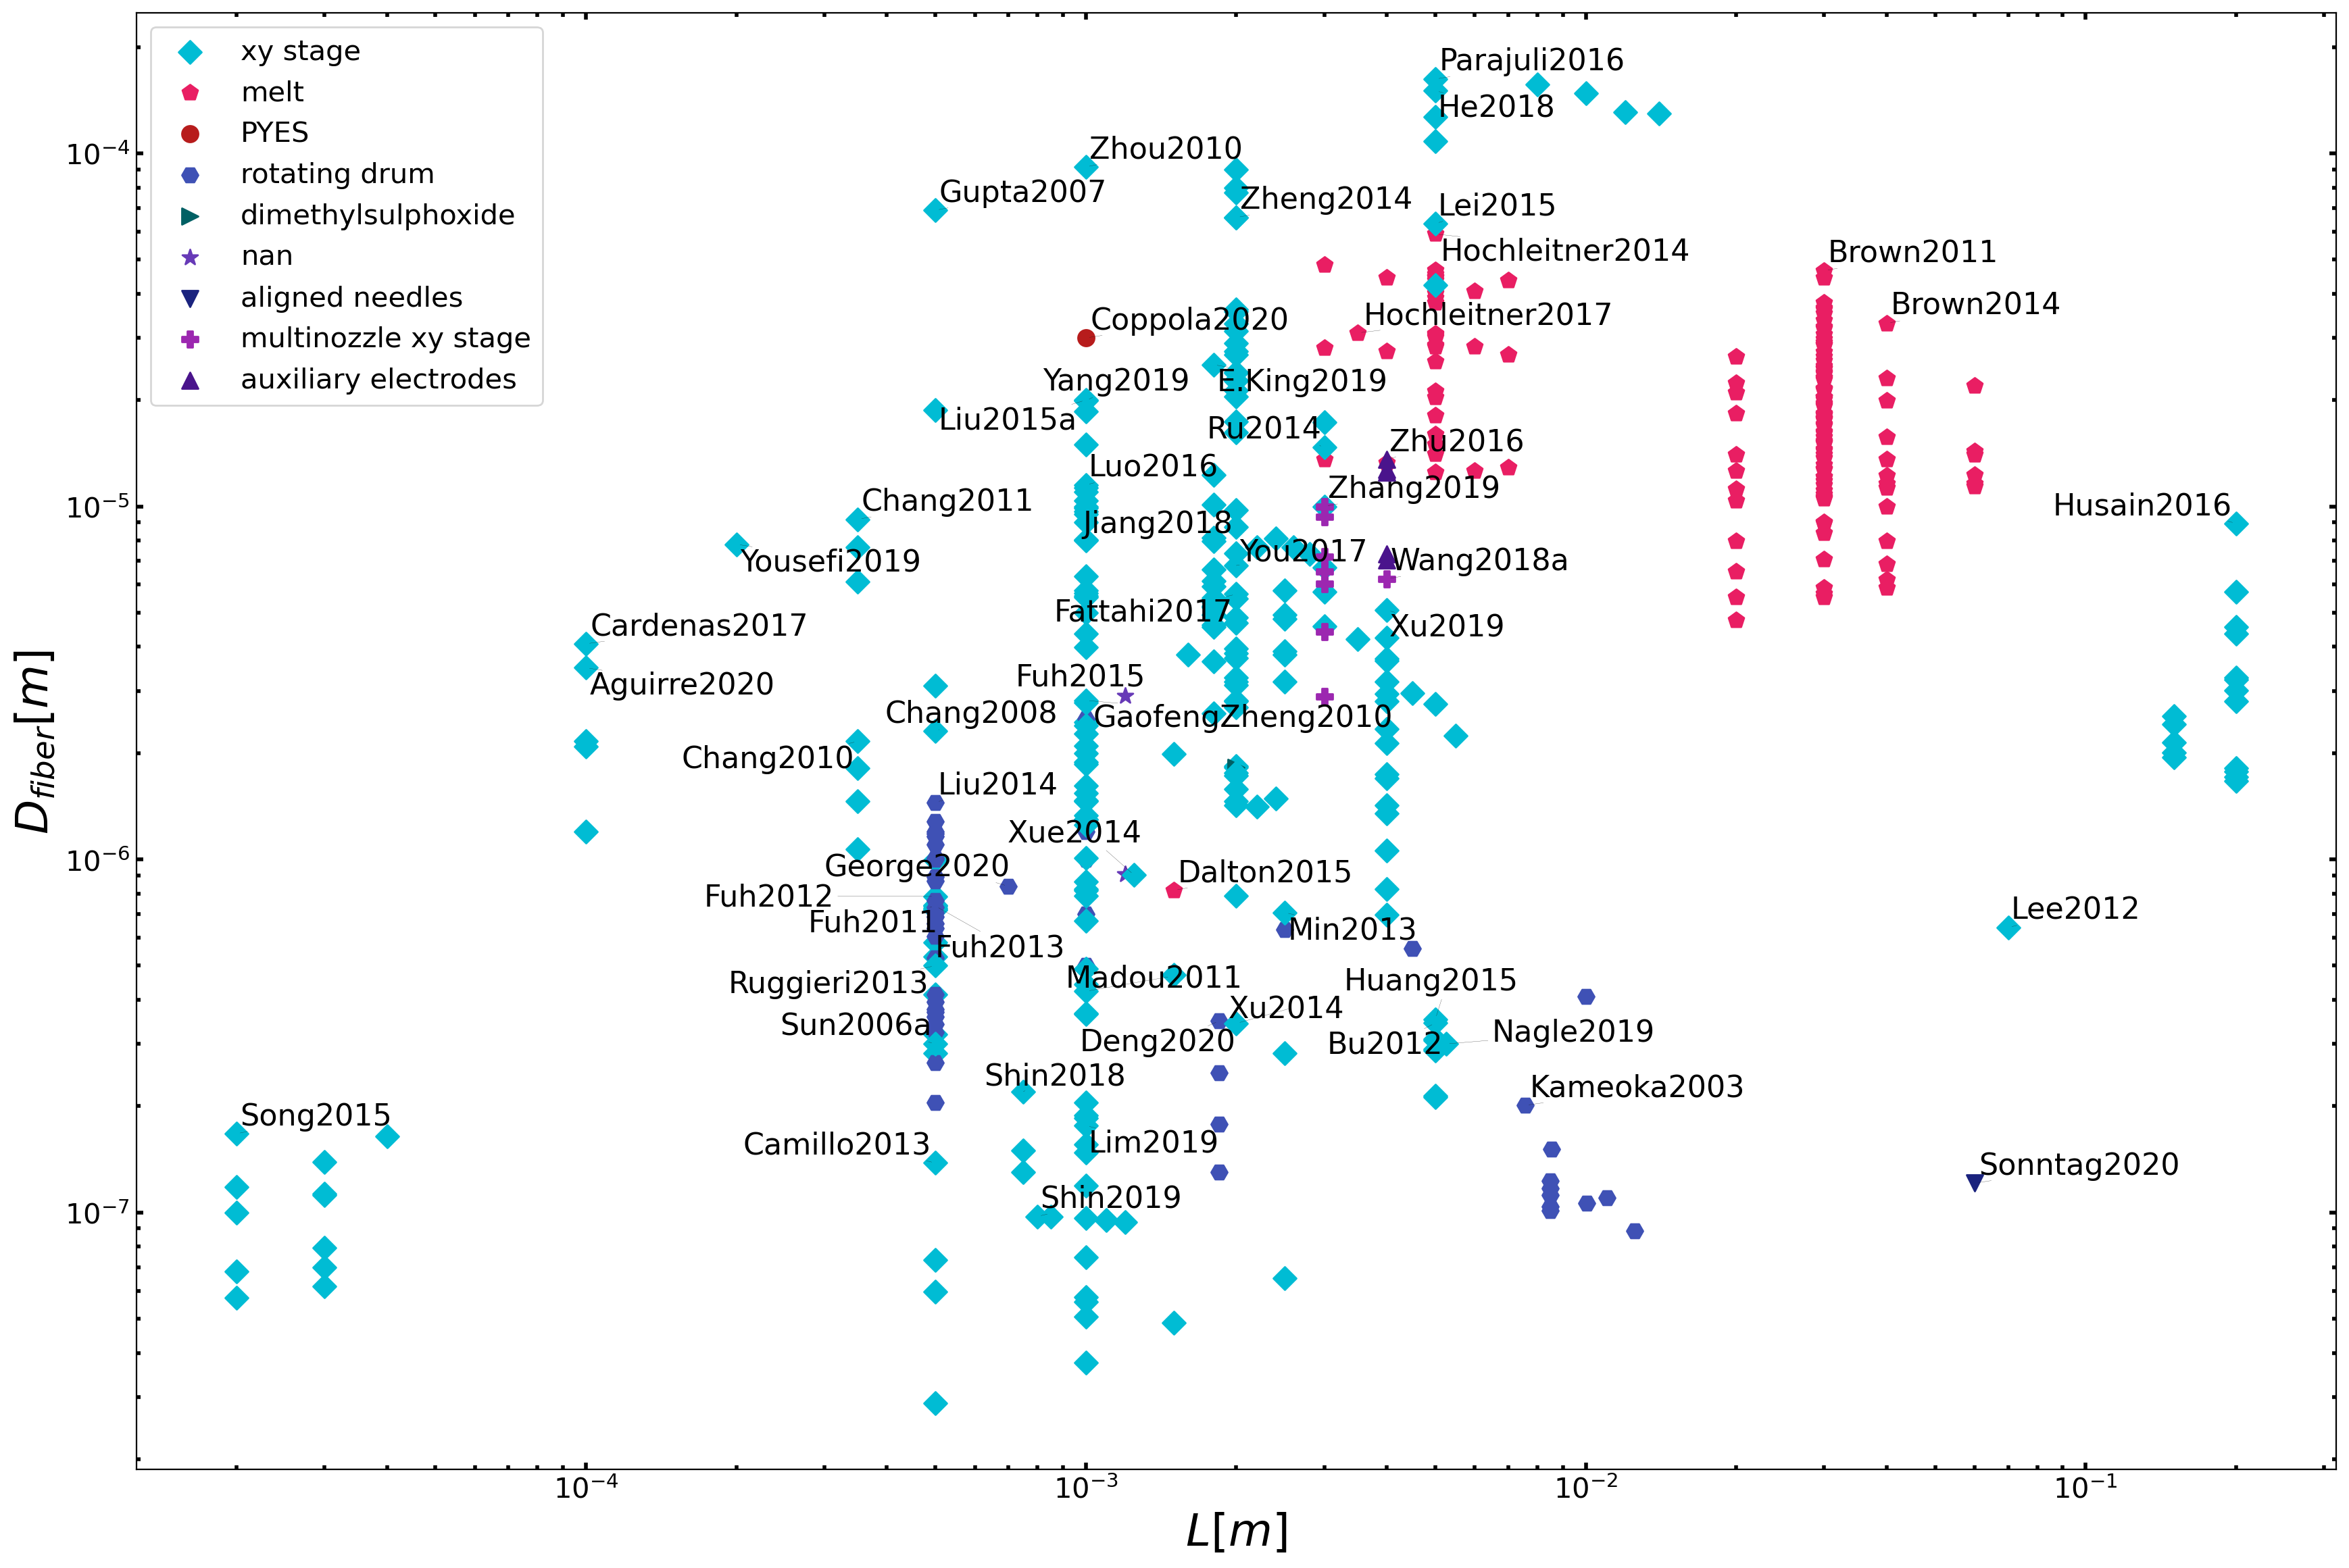
\includegraphics[width=\textwidth]{./Figures/plt_Lm_vs_Dfiberm.png}
\decoRule
\caption[Scatter Plot of NFES Working Distances and Fiber Diameters from Literature Experimental Results]{Scatter Plot of NFES Working Distances and Fiber Diameters from Literature Experimental Results. \cite{
  Yang2019,Fattahi2017,Shin2019,Wang2015,Parajuli2016,Zheng2010,Fuh2011,Dalton2015,
  Ru2014,Xue2014,Wang2017,Xu2014,Liu2013,Pan2014,Canton2014,Chakraborty2009,Gupta2007,
  He2018,Zhou2011,Chen2013,Williams2018,Choi2017,Pan2019,Lei2015,Lim2019,Park2020,
  Fuh2012,Flores2017,Chang2010,Xu2019,Zhang2019,Shin2018,Fuh2015,Nagle2019,Zheng2012,
  Kameoka2003a,Liu2014,E.King2019,Hochleitner2017,Madou2011,Jiang2018,Husain2016,
  ElectrospinTech2015,Brown2011,Kolan2018,Chang2011,Beachley2011,Camillo2013,Kameoka2003,
  Bu2012,Lee2012,Huang2015,Coppola2020,CisquellaSerra2019,Ruggieri2013,Hochleitner2014,
  Zhu2016,Brown2014,Chang2008,Sonntag2020,Kim2018,Deng2020,Han2019,George2020,Sun2006a,
  Pan2015,Shen2016,Strauss2019,Fuh2013,Sarkar2007,You2017,Wang2018a,Zheng2014,Song2015,
  GaofengZheng2010,Liu2015a,Min2013,Luo2016,Yousefi2019,Cardenas2017,Coppola2014}}
\label{fig:plt_Lm_vs_Dfiberm}
\end{figure}

\begin{figure}[!th]
\centering
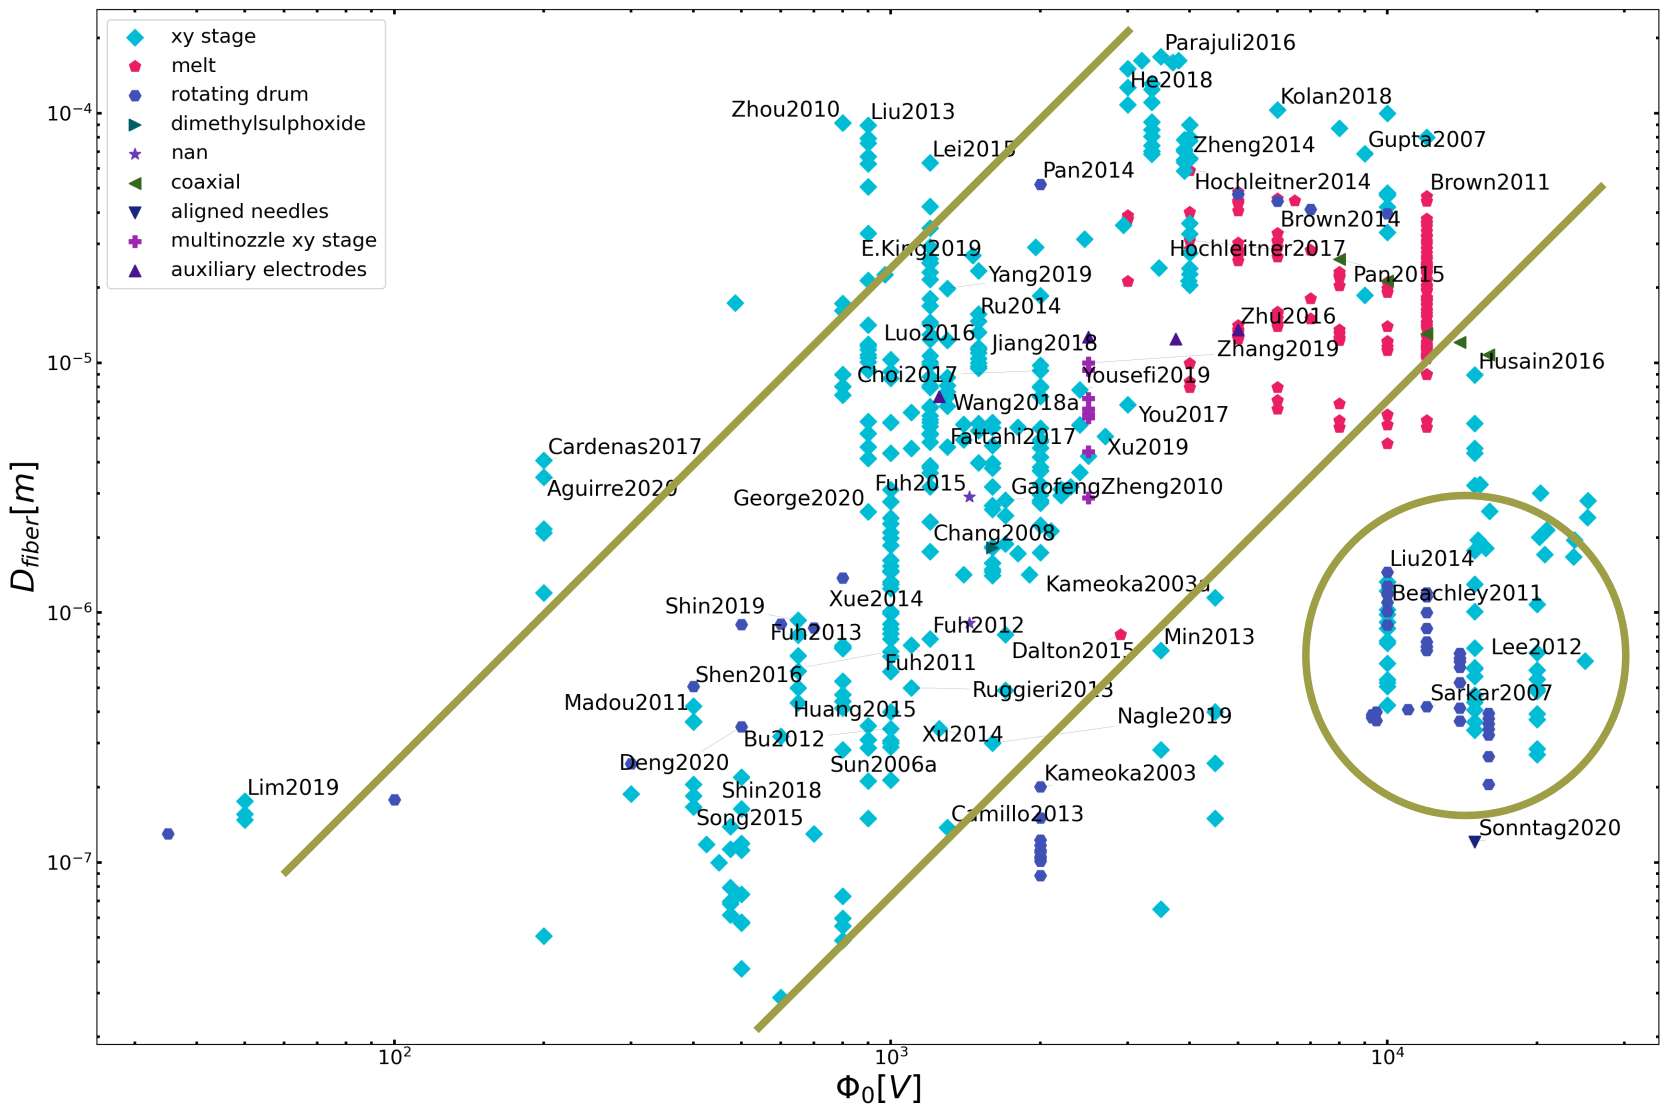
\includegraphics[width=\textwidth]{./Figures/plt_Phi0V_vs_Dfiberm.png}
\decoRule
\caption[Scatter Plot of NFES Applied Voltages and Fiber Diameters from Literature Experimental Results]{Scatter Plot of NFES Applied Voltages and Fiber Diameters from Literature Experimental Results. \cite{
  Yang2019,Fattahi2017,Shin2019,Wang2015,Parajuli2016,Zheng2010,Fuh2011,Dalton2015,
  Ru2014,Xue2014,Wang2017,Xu2014,Liu2013,Pan2014,Canton2014,Chakraborty2009,Gupta2007,
  He2018,Zhou2011,Chen2013,Williams2018,Choi2017,Pan2019,Lei2015,Lim2019,Park2020,
  Fuh2012,Flores2017,Chang2010,Xu2019,Zhang2019,Shin2018,Fuh2015,Nagle2019,Zheng2012,
  Kameoka2003a,Liu2014,E.King2019,Hochleitner2017,Madou2011,Jiang2018,Husain2016,
  ElectrospinTech2015,Brown2011,Kolan2018,Chang2011,Beachley2011,Camillo2013,Kameoka2003,
  Bu2012,Lee2012,Huang2015,Coppola2020,CisquellaSerra2019,Ruggieri2013,Hochleitner2014,
  Zhu2016,Brown2014,Chang2008,Sonntag2020,Kim2018,Deng2020,Han2019,George2020,Sun2006a,
  Pan2015,Shen2016,Strauss2019,Fuh2013,Sarkar2007,You2017,Wang2018a,Zheng2014,Song2015,
  GaofengZheng2010,Liu2015a,Min2013,Luo2016,Yousefi2019,Cardenas2017,Coppola2014}}
\label{fig:plt_Phi0V_vs_Dfiberm}
\end{figure}



\begin{figure}[!th]
\centering
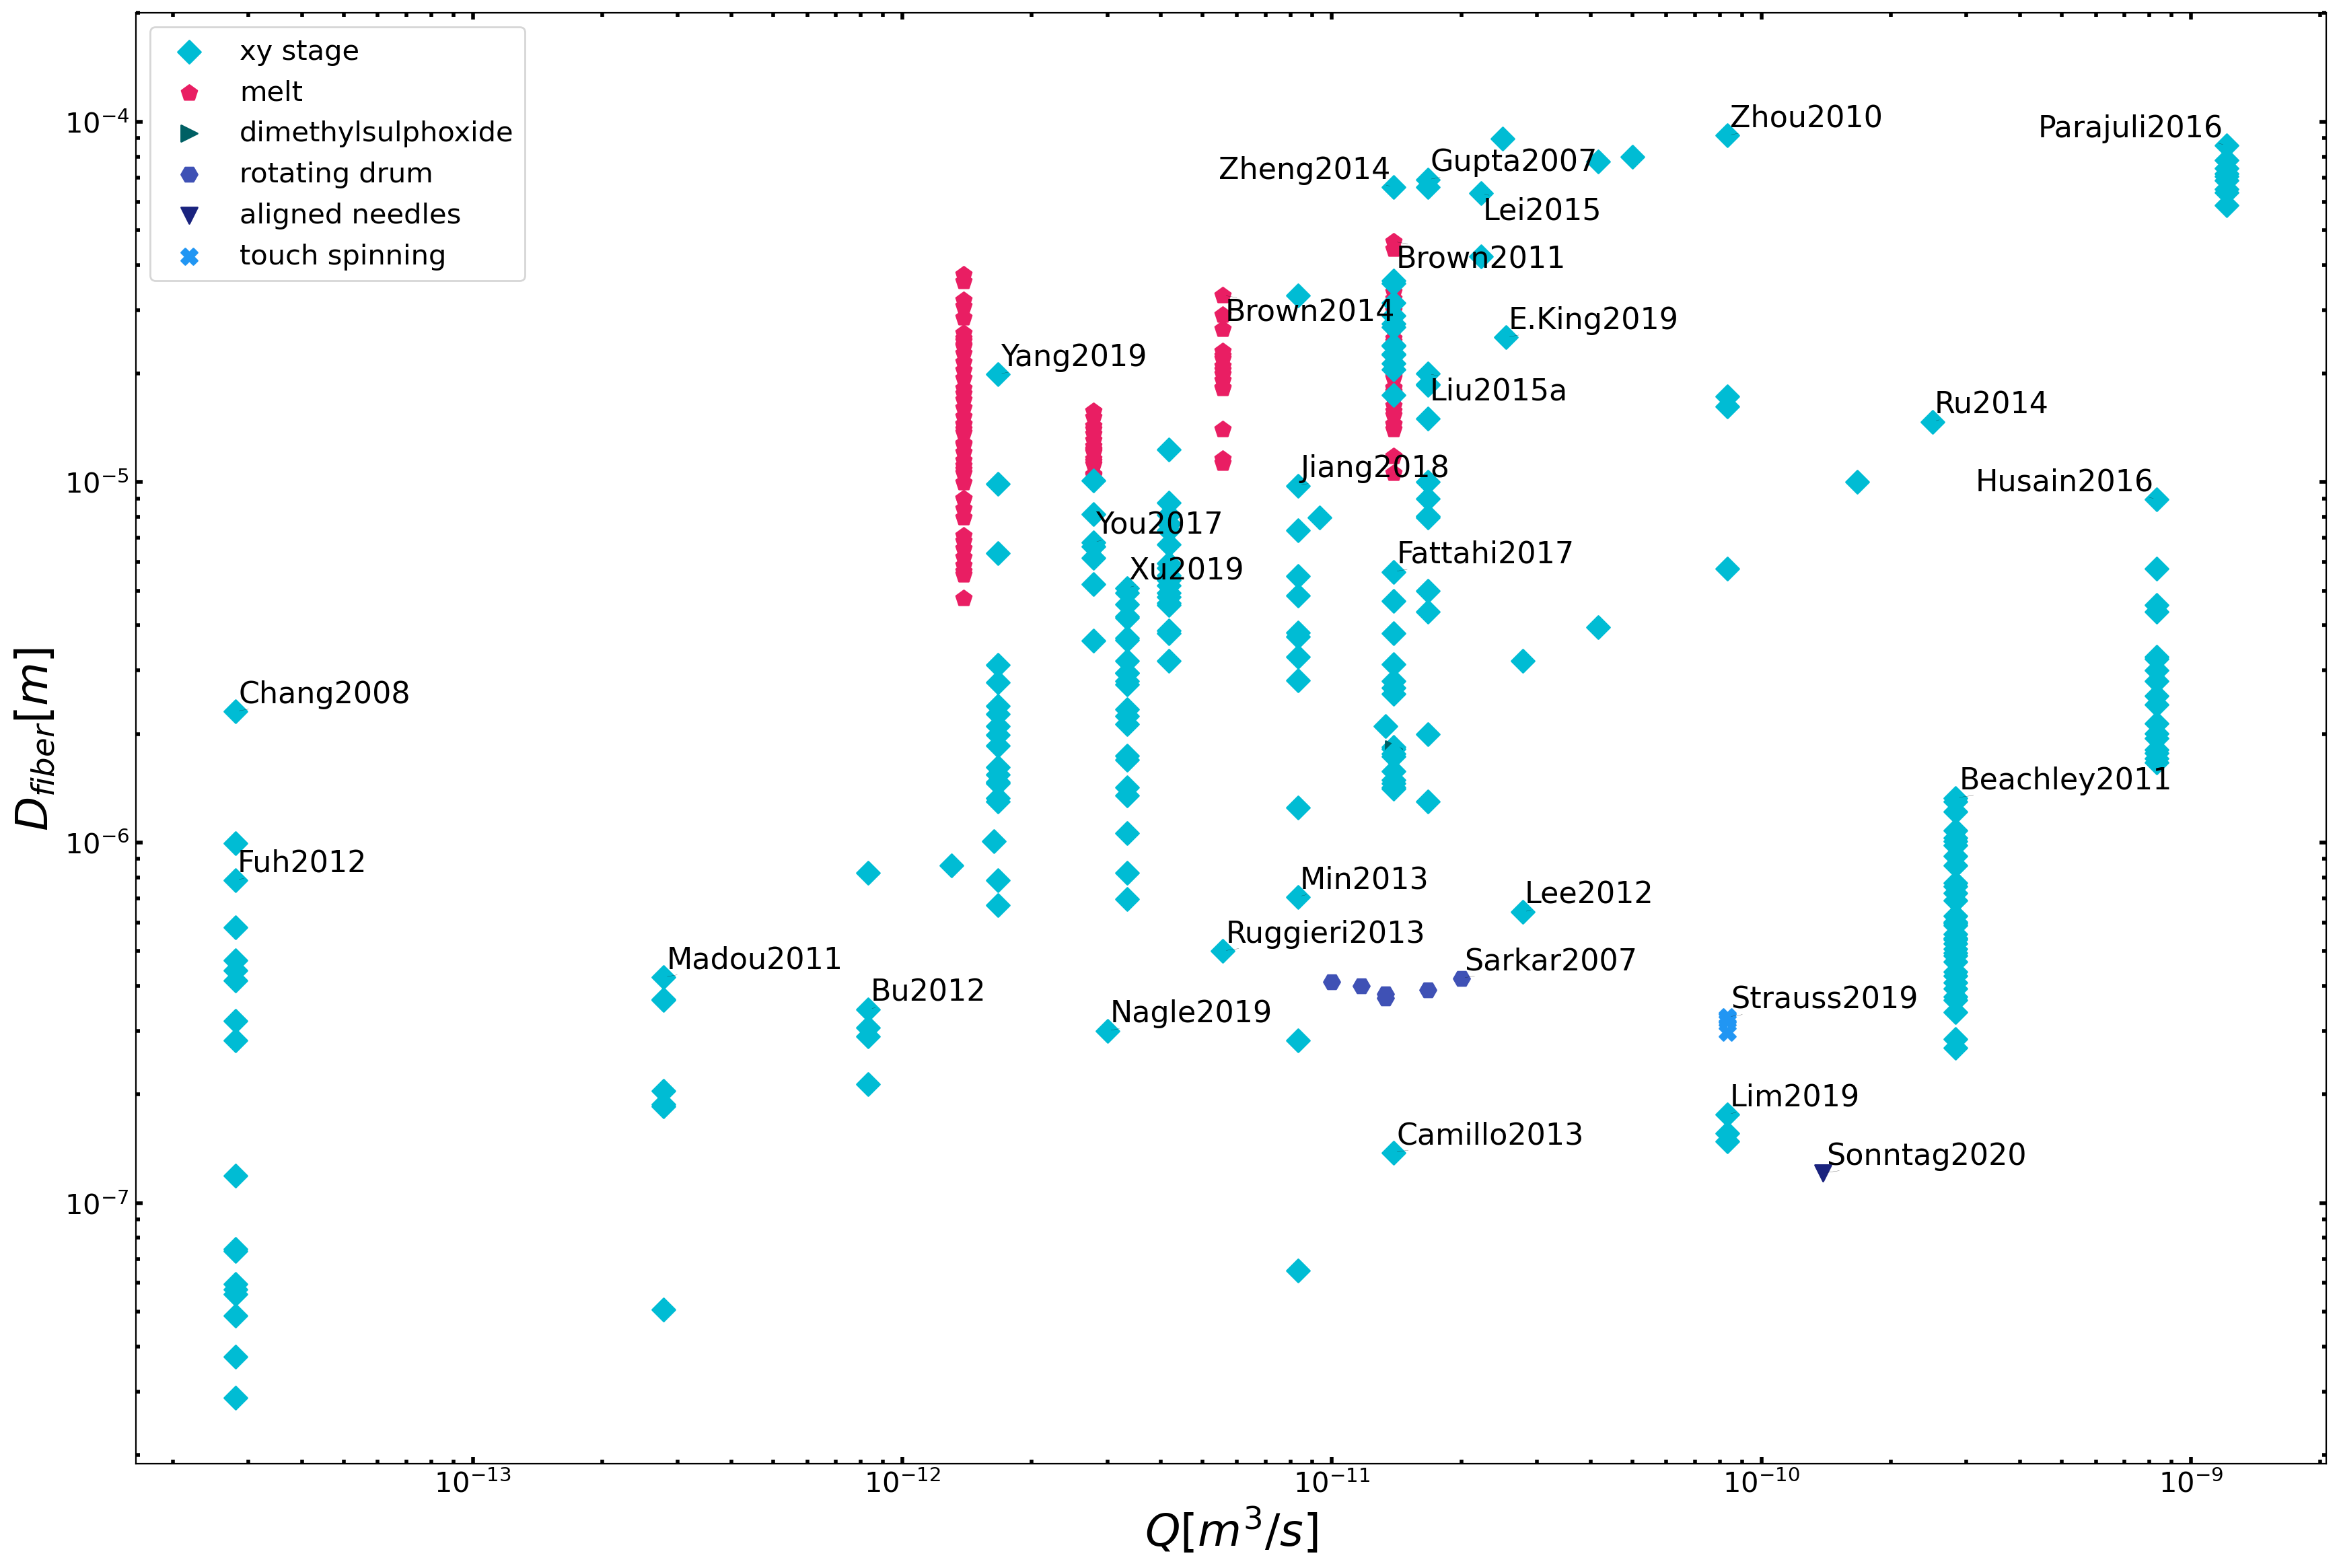
\includegraphics[width=\textwidth]{./Figures/plt_Qm3s_vs_Dfiberm.png}
\decoRule
\caption[Scatter Plot of Polymer Solution Flow Rates and Fiber Diameters from Literature Experimental Results]{Scatter Plot of Polymer Solution Flow Rates and Fiber Diameters from Literature Experimental Results. \cite{
  Yang2019,Fattahi2017,Shin2019,Wang2015,Parajuli2016,Zheng2010,Fuh2011,Dalton2015,
  Ru2014,Xue2014,Wang2017,Xu2014,Liu2013,Pan2014,Canton2014,Chakraborty2009,Gupta2007,
  He2018,Zhou2011,Chen2013,Williams2018,Choi2017,Pan2019,Lei2015,Lim2019,Park2020,
  Fuh2012,Flores2017,Chang2010,Xu2019,Zhang2019,Shin2018,Fuh2015,Nagle2019,Zheng2012,
  Kameoka2003a,Liu2014,E.King2019,Hochleitner2017,Madou2011,Jiang2018,Husain2016,
  ElectrospinTech2015,Brown2011,Kolan2018,Chang2011,Beachley2011,Camillo2013,Kameoka2003,
  Bu2012,Lee2012,Huang2015,Coppola2020,CisquellaSerra2019,Ruggieri2013,Hochleitner2014,
  Zhu2016,Brown2014,Chang2008,Sonntag2020,Kim2018,Deng2020,Han2019,George2020,Sun2006a,
  Pan2015,Shen2016,Strauss2019,Fuh2013,Sarkar2007,You2017,Wang2018a,Zheng2014,Song2015,
  GaofengZheng2010,Liu2015a,Min2013,Luo2016,Yousefi2019,Cardenas2017,Coppola2014}}
\label{fig:plt_Qm3s_vs_Dfiberm}
\end{figure}

\begin{figure}[!th]
\centering
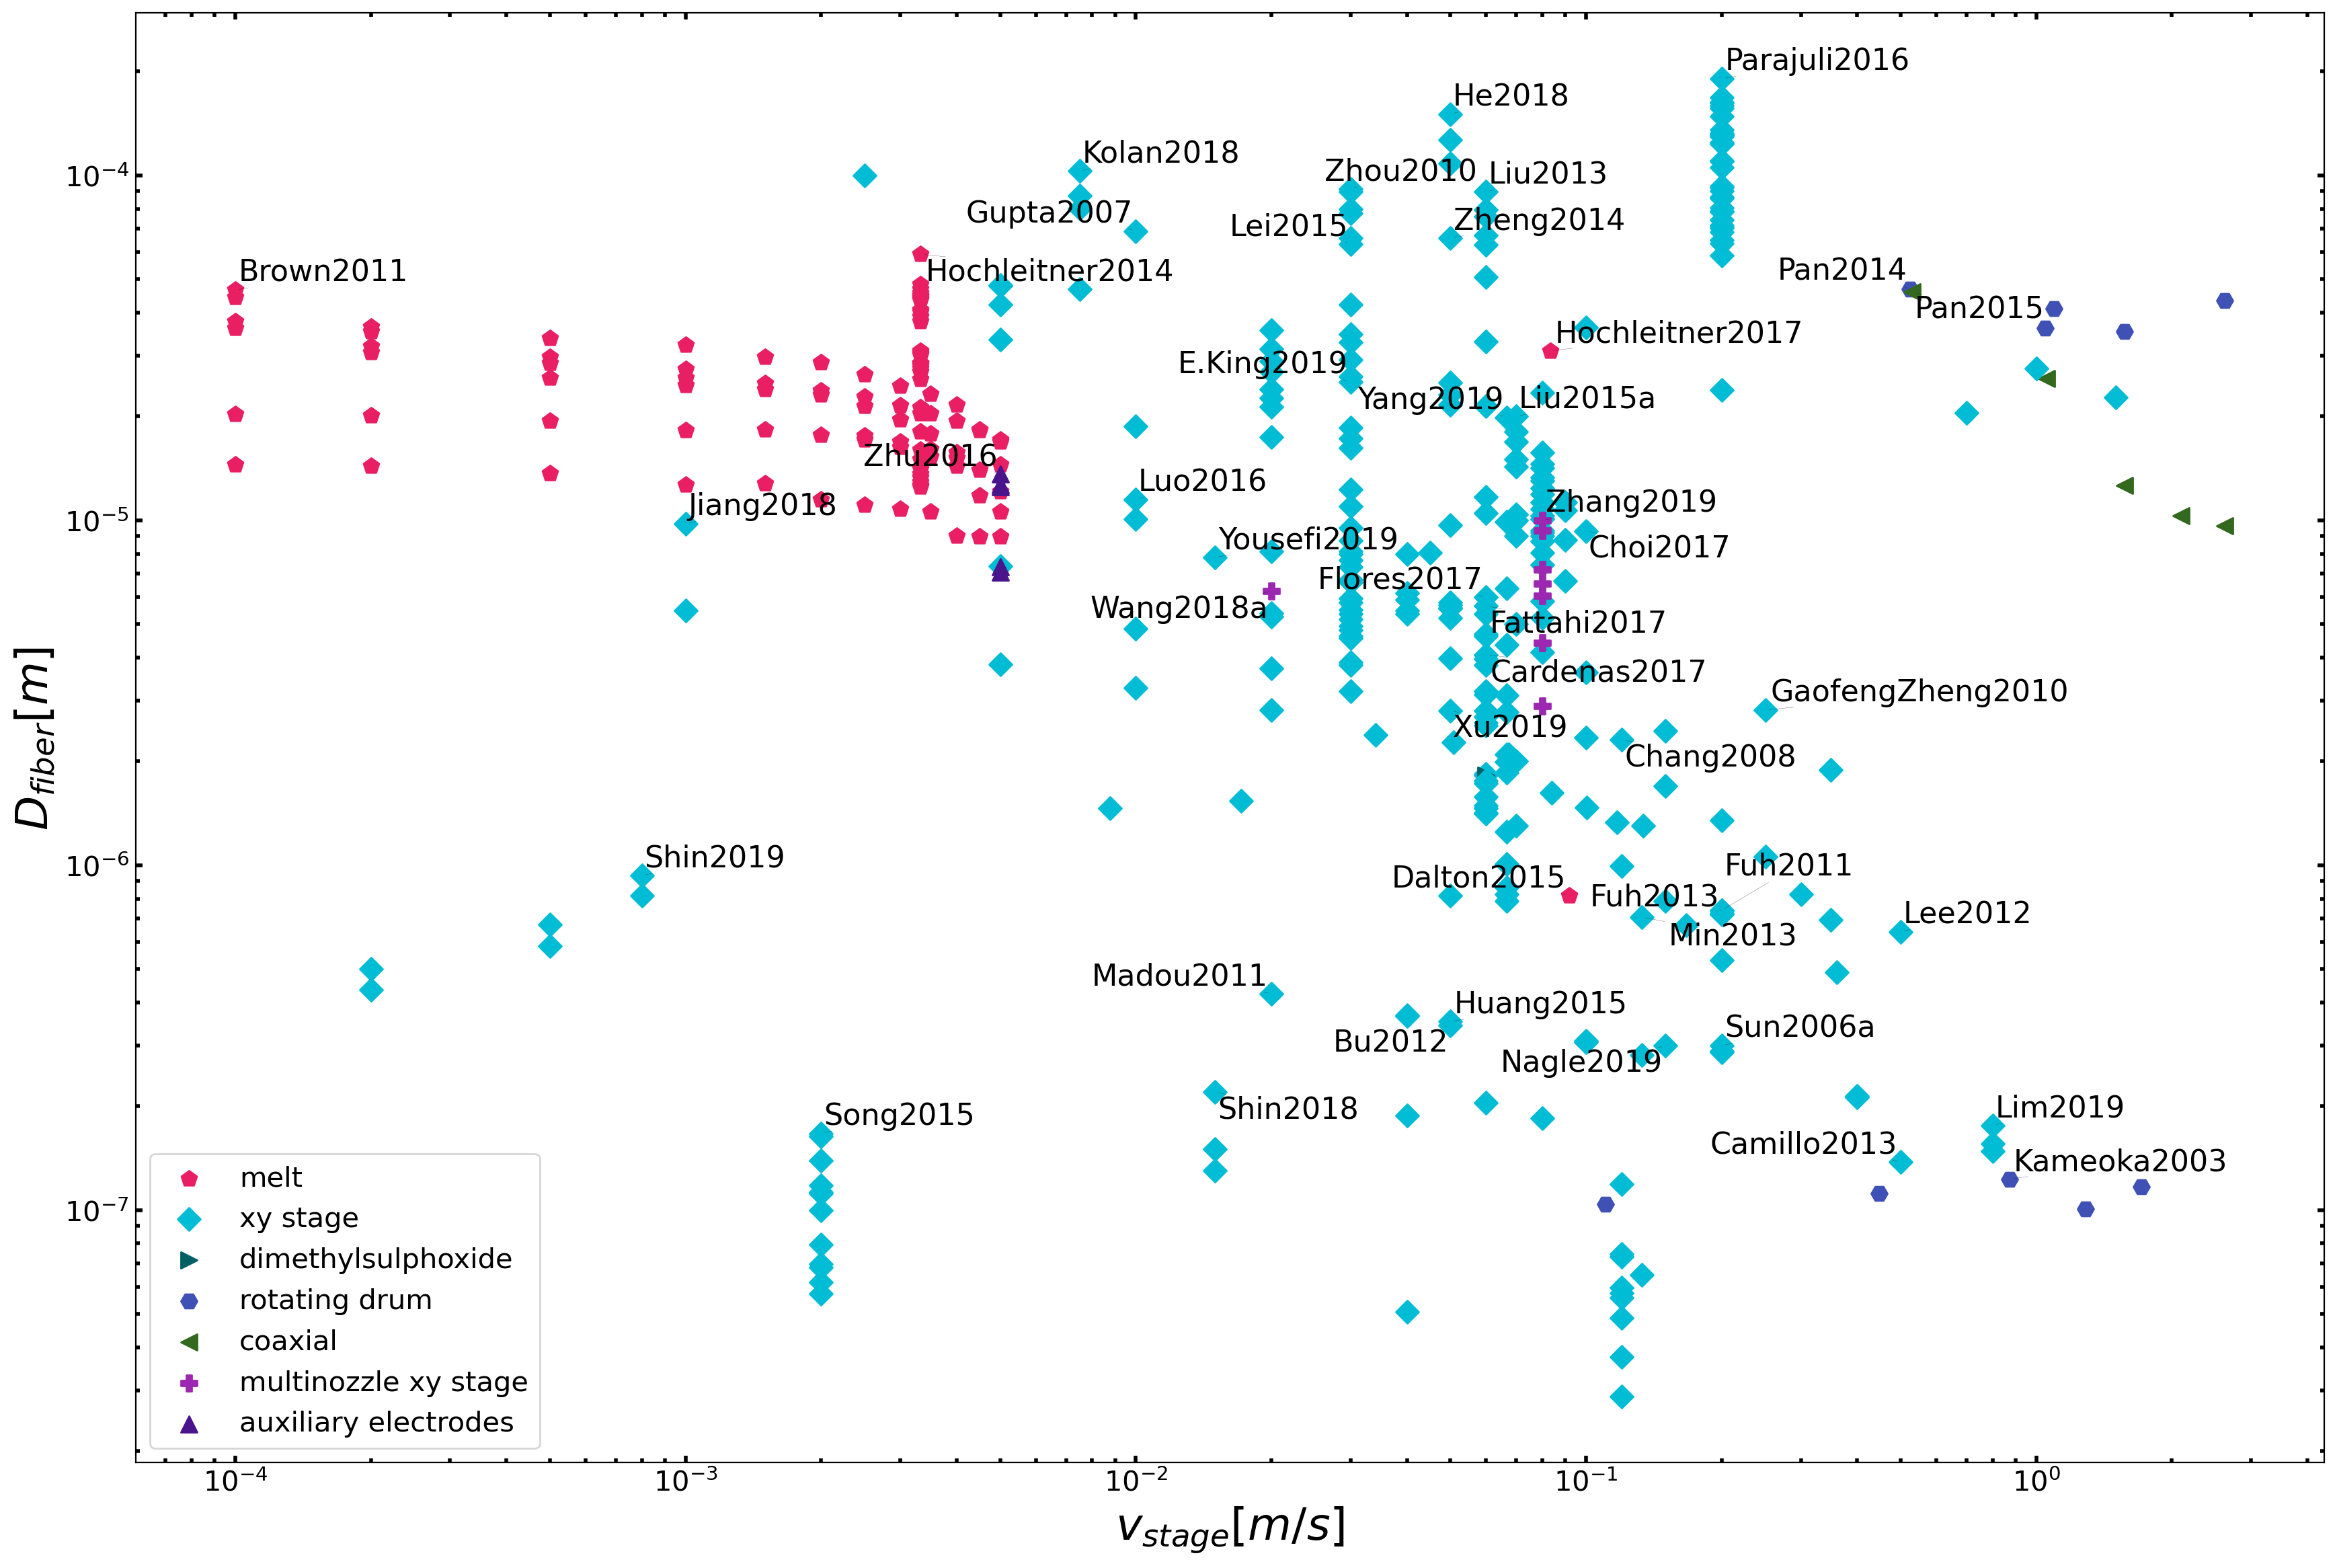
\includegraphics[width=\textwidth]{./Figures/plt_vstagems_vs_Dfiberm.png}
\decoRule
\caption[Scatter Plot of Collector xy Stage Velocities and Fiber Diameters from Literature Experimental Results]{Scatter Plot of Collector xy Stage Velocities and Fiber Diameters from Literature Experimental Results. \cite{
  Yang2019,Fattahi2017,Shin2019,Wang2015,Parajuli2016,Zheng2010,Fuh2011,Dalton2015,
  Ru2014,Xue2014,Wang2017,Xu2014,Liu2013,Pan2014,Canton2014,Chakraborty2009,Gupta2007,
  He2018,Zhou2011,Chen2013,Williams2018,Choi2017,Pan2019,Lei2015,Lim2019,Park2020,
  Fuh2012,Flores2017,Chang2010,Xu2019,Zhang2019,Shin2018,Fuh2015,Nagle2019,Zheng2012,
  Kameoka2003a,Liu2014,E.King2019,Hochleitner2017,Madou2011,Jiang2018,Husain2016,
  ElectrospinTech2015,Brown2011,Kolan2018,Chang2011,Beachley2011,Camillo2013,Kameoka2003,
  Bu2012,Lee2012,Huang2015,Coppola2020,CisquellaSerra2019,Ruggieri2013,Hochleitner2014,
  Zhu2016,Brown2014,Chang2008,Sonntag2020,Kim2018,Deng2020,Han2019,George2020,Sun2006a,
  Pan2015,Shen2016,Strauss2019,Fuh2013,Sarkar2007,You2017,Wang2018a,Zheng2014,Song2015,
  GaofengZheng2010,Liu2015a,Min2013,Luo2016,Yousefi2019,Cardenas2017,Coppola2014}}
\label{fig:plt_vstagems_vs_Dfiberm}
\end{figure}


The effect of parameters such as ink concentration, working distance, applied voltage, and stage speed on the diameter of the printed nano-fibers was investigated, a summary is presented in Table \ref{tab:nfesProcessParameters}.

\begin{table}[ht]
\centering
\caption[Near-Field Electrospinning Process Parameters]{Summary of the main parameters that drive the electrospinning process, ordered by: polymer solution parameters, process parameters, and ambient parameters. Adapted from \cite{Bagbi2019, Unnithan2015}}
\begin{tabularx}{\textwidth}{lX}
\hline
\textbf{NFES Process Parameters} & \textbf{Effect} \\
\hline
\textbf{Solution Parameters:} &  \\
Concentration & Concentration shall be high enough to produce uniform nano-fibers, but low enough to prevent nozzle clogging \\
Molecular weight & High-molecular-weight polymers yield smoother fibers \\
Viscosity & Zero-shear viscosity shall be optimal to generate a constant jet from the needle \\
Conductivity & Solution shall be conductive enough for the electric field to have influence on the jet \\
\textbf{Process Parameters:} &  \\
Applied voltage & Higher voltages eject more material from the nozzle \\
Flow rate & Slow flow rates yield thinner fibers, but it shall be fast enough to prevent clogging and keep the Taylor cone in a constant size and shape \\
Working distance & Long distances result in thinner fibers, however the spatial control is hampered \\
\textbf{Ambient Parameters:} &  \\
Humidity & Increasing humidity produces thicker diameters \\
Temperature & Increasing temperature yields thinner fibers, however high temperatures make the nozzle prone to clog as the solvent evaporates at a faster rate \\
\hline
\end{tabularx}
\label{tab:nfesProcessParameters}
\end{table}

\section{Diameter Prediction of Electrospun Fibers} % adimensional analysis

Electrospinning is a simple process to fabricate fibers of different diameters. However, the final diameter of a fiber depends on various solution, process, and ambient parameters (Table \ref{tab:nfesProcessParameters}) with interaction with rheology and fluid dynamics. Given the connection of various parameters, it is not trivial to derive a mathematical model to describe the complete electrospinning process. Current attempts involve limited models that can only describe the steady jet region for specific polymer solutions. \cite{Hohman2001a,Feng2002a,Reneker2000} From literature \cite{Greiner2008, Deitzel2001, Cui2007, Beachley2011} and as described in Figure \ref{fig:plt_corMat}, zero-shear viscosity, flow rate and applied voltage are the main drivers that determine the final fiber morphology and dimensions. Other parameters such as solution surface tension, conductivity and working distance have less impact on the electrospun fibers. \cite{Ramakrishna2005} As shown in Figures \ref{fig:plt_Qm3s_vs_Dfiberm} and \ref{fig:plt_Cpolymerwt_vs_Dfiberm}, literature states that flow rate $Q$ and solution concentration $C_{polymer}$ are directly proportional to the fiber diameter $D_{fiber}$. \cite{Wang2008, McKee2004, Gupta2005}

As mentioned in the previous section, the correlation between the final fiber diameter $D_{fiber}$ and the applied voltage $\Phi_0$ is not well understood. Most authors posit that the fiber diameter decreases with increasing voltage. \cite{Yuan2004, Wang2009, Thompson2007, Sajeev2008, Mazoochi2011, MATARAM2011, Liu2007, Homayoni2009, Zhang2005} Nevertheless, other publications state the inverse correlation. \cite{Rojas2009, Jeun2007} This discrepancy between the final fiber diameter $D_{fiber}$ and the applied voltage $\Phi_0$ may be attributed to the fact that $\Phi_0$ is also related to the electric field $\Phi_0 / L$, which in turn is related to the working distance $L$. As the electric field $\Phi_0 / L$ increases, the electric field forces loose influence under the polymer jet as the increased force results into faster evaporation of the solvent promoting faster solidification. On the other hand, polymer concentration $C_{polymer}$, and conductivity $K$ also have an effect on the electric field. \cite{Thompson2007, Mohan2002} 

On the other hand, Zhang et al., Kim et al., and Mituppatham et al. studied the relationship between the solution surface tension $\gamma$ and its conductivity $K$. \cite{Zhang2005, Kim2005, Mituppatham2004} Kim's and Mituppatham report a increase in fiber diameter with increasing conductivity in the polymer solution, while Zhang reports the inverse relationship. The existing interdependence between the process and solution parameters adds complexity and ambiguity to the effect of each parameter. The fiber morphology not only depends on the process parameters, but also on the type of electrospinning process and on polymer-solvent system. \cite{Gadkari2014}

Helgeson and Wagner \cite{Helgeson2007} have presented a dimension-less analysis to predict the fiber diameter with conservation equations of momentum, mass, electric charge and four dimensionless numbers: Peclet number $ \displaystyle Pe = \frac{2 \bar{\varepsilon} v_0}{K R_0} $, Reynold number $ \displaystyle Re = \frac{\rho v_0 R_0}{\eta_0} $, Weber number $ \displaystyle We = \frac{\rho {v_0}^2 R_0}{\gamma} $, and the dimensionless electric field strength $ \displaystyle \Psi = \frac{\bar{\varepsilon} {E_0}^2}{\rho {v_0}^2} $. Where $\bar{\varepsilon}$ is the dielectric permitivity of the atmosphere, $K$ the solution conductivity, $\rho$ the density, $\eta_0$ the zero-shear viscosity, $\gamma$ the surface tension, $E_0$ the applied electric field, $R_0$ the initial jet radius, and $v_0$ the initial jet velocity. Since $R_0$ and $v_0$ can neither be controlled nor measured, Helgeson arrived to a correlation between the electrostatic and viscous forces $\Pi_1$ describing the stress directing the polymer jet elongation from the source to the collector plate. \cite{Helgeson2007}

\begin{equation}\label{eqn:electroViscousRatio}
    \Pi_1 = Re Pe \Psi = \frac{2 {\bar{\varepsilon}}^2 {\Phi_0}^2}{K \eta_0 L^2}
\end{equation}

the Ohnesorge number, resulting from the manipulation of the Reynolds number $Re$ and the Weber number $We$, is used to explain the behavior of the polymeric solution jet under small disturbances, due the presence of a voltage, leading to the capillary rupture of the fluid jet. \cite{Helgeson2007}

\begin{equation}\label{eqn:ohnesorgeNumber}
    Oh = \frac{{Re}^2}{We} = \frac{\eta_0}{\sqrt{\rho \gamma R_{jet}}}
\end{equation}

Where $ \displaystyle R_{jet} = R_f \sqrt{\frac{1}{w_s}} $ is the wet radius of the jet solution, which is calculated from the radius of the dry fiber $R_f$ and the mass fraction of the polymer in solution $w_s$. \cite{Helgeson2007}

\begin{figure}[!th]
\centering
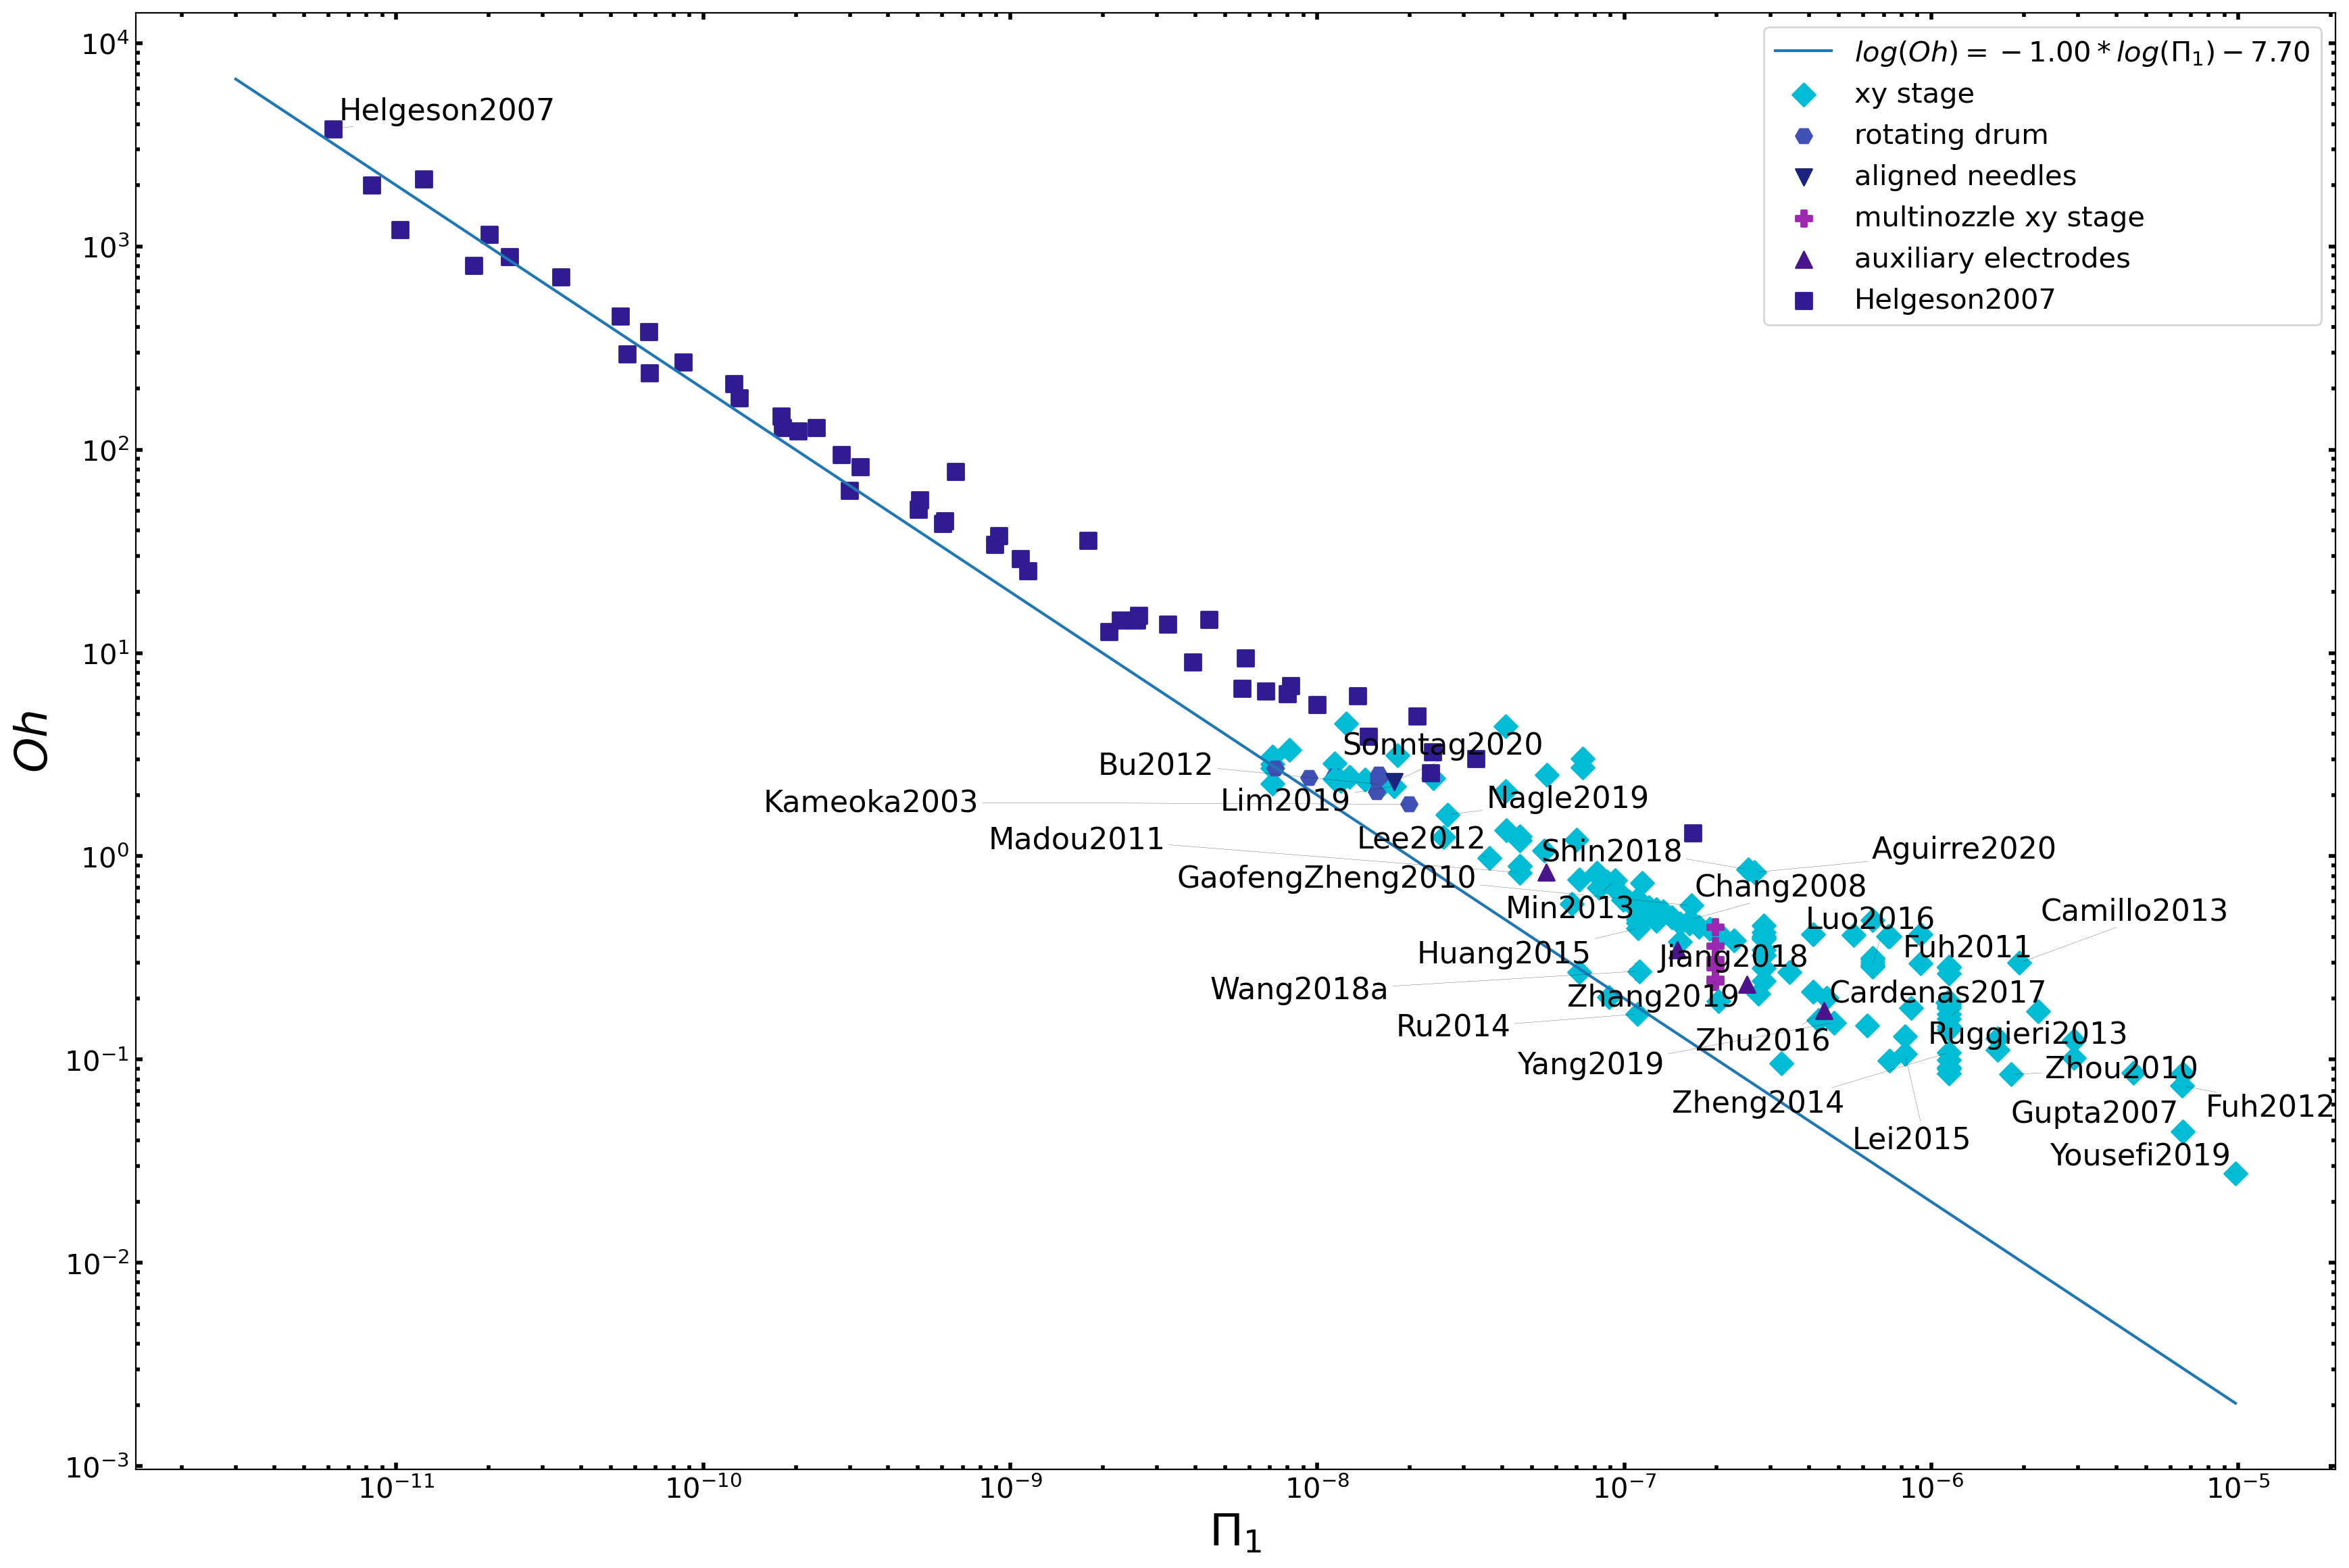
\includegraphics[width=\textwidth]{./Figures/plt_Pi1_vs_Oh.png}
\decoRule
\caption[Image Analysis Algorithm to Measure Fiber Diameters from SEM images]{Image Analysis Algorithm to Measure Fiber Diameters from SEM images. Ilustration uses Yousefi et al.'s work as an example. \cite{Helgeson2007,
  Yang2019,Fattahi2017,Shin2019,Wang2015,Parajuli2016,Zheng2010,Fuh2011,Dalton2015,
  Ru2014,Xue2014,Wang2017,Xu2014,Liu2013,Pan2014,Canton2014,Chakraborty2009,Gupta2007,
  He2018,Zhou2011,Chen2013,Williams2018,Choi2017,Pan2019,Lei2015,Lim2019,Park2020,
  Fuh2012,Flores2017,Chang2010,Xu2019,Zhang2019,Shin2018,Fuh2015,Nagle2019,Zheng2012,
  Kameoka2003a,Liu2014,E.King2019,Hochleitner2017,Madou2011,Jiang2018,Husain2016,
  ElectrospinTech2015,Brown2011,Kolan2018,Chang2011,Beachley2011,Camillo2013,Kameoka2003,
  Bu2012,Lee2012,Huang2015,Coppola2020,CisquellaSerra2019,Ruggieri2013,Hochleitner2014,
  Zhu2016,Brown2014,Chang2008,Sonntag2020,Kim2018,Deng2020,Han2019,George2020,Sun2006a,
  Pan2015,Shen2016,Strauss2019,Fuh2013,Sarkar2007,You2017,Wang2018a,Zheng2014,Song2015,
  GaofengZheng2010,Liu2015a,Min2013,Luo2016,Yousefi2019,Cardenas2017,Coppola2014}}
\label{fig:plt_Pi1_vs_Oh}
\end{figure}

Figure \ref{fig:plt_Pi1_vs_Oh} plots the $\Pi_1$ and $Oh$ values reported by \cite{Helgeson2007} along with new data points from the data collection of NFES fiber diameters and process parameters. It is possible to observe the predominance of the viscous and the electrostatic forces within the solution by the magnitude $\Pi_1$ (Equation \ref{eqn:electroViscousRatio}). On the other hand $Oh$ (Equation \ref{eqn:ohnesorgeNumber}) reflects the capacity of the viscous forces over the polymeric jet, which allows stability in the electrospinning process. The data points gathered by Helgeson et al. are from far-field electrospinning studies, whereas the new data points belong to near-field electrospinning studies.

The analysis suggests that both types of electrospinning behave in a similar manner, where the FFES data fits better a linear behavior of slope $-1$. As the working distance closes in NFES, the data points fit a shallower slope with higher $\Pi_1$ values and lower $Oh$ values. This suggests that in NFES less viscous solutions have been used, since in long working distances a higher viscosity is needed to keep the integrity of the fiber in the whole traveling distance until it reaches the collector. For high $Oh$ values and elevated viscosity, the entanglement of the polymeric chains is higher, resulting in the formation of individual fibers; also, the jet is prone to faster solidification, due to an early evaporation of solvent, due to the resistance to the change of momentum, caused by the high viscosity in the polymeric solution, hence the need of higher voltages in FFES. Helgeson et al. suggest that the following relationship in Equation \ref{eqn:ohnesorgeNumberRelationship} can be used to predict the fiber diameter, as in the trend in Figure \ref{fig:plt_Pi1_vs_Oh} $Oh$ has an inverse linear relationship with $\Pi_1$. \cite{Helgeson2007}

\begin{equation}\label{eqn:ohnesorgeNumberRelationship}
    \Pi_1 Oh = \frac{2 {\bar{\varepsilon}}^2 {\Phi_0}^2}{K L^2 \sqrt{\rho \gamma R_{jet}}} = 2.5 \pm 0.2 \times 10^{-8}
\end{equation}

The absence of the solution zero-shear viscosity in Equation \ref{eqn:ohnesorgeNumberRelationship} suggests that $\eta_0$ by its own is insufficient to predict the fiber diameter. The solution conductivity, process parameters and surface tension are also needed to describe the diameter of electrospun fibers \cite{Helgeson2007}, as stated in section \ref{sec:parametersThatAffectTheDiameter}. Moreover, the viscosity term is embedded within the mass fraction of the polymer in solution $w_s$ in the $R_{jet}$ term. Finally, Equation \ref{eqn:ohnesorgeNumberRelationship} can be validated by the observations from the correlation matrix and scatter plots as the same parameters are present in both analyses with the same proportional relationship.